	
%%%%%%%%%%%% 3 %%%%%%%%%%%%%%%%%%%%%%%%%%%%%%%%%%%%%%%%%%%%%%%%%%%%%%%%%%%%%%%%%%%%%%%%%%%%%%%%%%%%%%%%%%%%%%%%%%%%%%%%%%%%%%
\chapter{Instrument Calibration}
%%%%%%%%%%%%%%%%%%%%%%%%%%%%%%%%%%%%%%%%%%%%%%%%%%%%%%%%%%%%%%%%%%%%%%%%%%%%%%%%%%%%%%%%%%%%%%%%%%%%%%%%%%%%%%%%%%%%%%%%%%%%

	The ANITAIII digitizing electronics require calibration in order to relate recorded digital signals to an analog electromagnetic field, and possible physics event, being measured.  There are several major considerations that must be taken into account in order to relate the recorded values to physical electromagnetic phenomena.  The LAB3 reports values in ADC counts, which need to be scaled to represent voltage at the input to the chip.  The sampling time base must be measured to determine its non-uniformity and correct for it after digitization.  The gain and phase effect of the signal chain impulse response must be deconvolved to determine the absolute electromagnetic field present at the detector.  Precision spacing of the antenna phase centers must be determined for accurate interferometric pointing and mapping, and for coherently summing waveforms. The in flight trigger efficiency of the system must be found. Data taken both on the ground and in flight is used to determine the calibration of the ANITAIII instrument. The following chapter details the steps taken and results of calibrating these aspects of the ANITAIII instrument.
	

	
\section{LABRADOR voltage calibration}
		The LAB3 ASIC, as described in Chapter 2, uses an SCA to store many sequential snapshots of the charge on a capacitor from a time varying electrical potential arriving at the chip.  This captured analog charge is then digitized (an analog to digital conversion, or ADC) utilizing a Wilkinson ADC, which compares the voltage to a constant current source voltage ramp signal that stops a Gray code counter at the time of comparator activation (see Figure \ref{fig:Lab_Digitization}.  The digital values read out by the acquisition software are thus a measurement of the time between when the ramp signal begins and when its voltage passes the voltage of the stored charged in that particular SCA bin.  This ADC count must be converted into a voltage that can be propagated back through the signal chain and inform us on the induced potential on the antenna.

\begin{figure}
	\includegraphics[width=\textwidth]{figures/LAB_Digitization}
	\caption{Simplified diagram of the digitization chain for the LABRADOR3 digitizer}
	\label{fig:Lab_Digitization}
\end{figure}	
		
	\subsection{Chip to Chip Variation}
		Each chip suffers from manufacturing process parameter spread introduced in the nano-lithography process.  Due to this, each chip must be calibrated independently.  The time base generator, the write pointer strobe propagation and RCO phase dependance, as well as the ADC to absolute voltage values must all be independently measured for each chip. 

	\subsection{Pedestal Subtraction}
		The signal propagated through the ANITAIII system is AC-coupled by design, and as such, must have a DC offset reintroduced to it before being coupled to the SCA within the LABRADOR.  The ramp voltage and comparator internal to the chip operate only at positive voltages (0 to 2.0V), and so, to get a measurement of both positive and negative voltage fluctuations, the signal must nominally be set at mid-range of the ramp signal, or about 1.0V.  This is accomplished through a fixed voltage regulator external to the LABRADOR on the SURF board.  This ``pedestal'' voltage, visible in the data as a constant ADC count offset, must be later subtracted to correctly zero mean the signal.  A ``pedestal run,'' in which large numbers of samples were measured and averaged to determine a mean value per capacitor bin, was done at the beginning of the flight and stored to the redundant storage drives.  These pedestals are then subtracted immediately after being read by the acquisition software (Acqd) before being stored, and are thus included in the raw data.  The pedestals used in ANITAIII are plotted in Figure \ref{fig:pedestals}
		
\begin{figure}
	\centering
	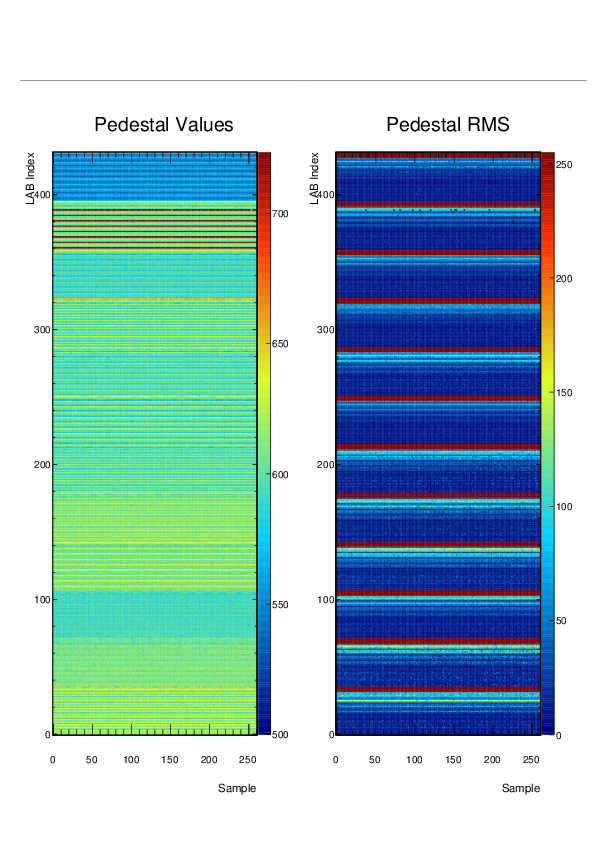
\includegraphics[height=0.8\textheight]{figures/Pedestals_big2}
	\caption{Mean pedestal values used for subtraction(left) and RMS of bin in pedestal run (right) for all LABRADOR chips for the ANITAIII flight.  The Y axis is an index describing the LABRADOR in question (SURF*36 + Chan*4 + LAB).  The X axis is the capacitor bin number within that surf.  The Z color axis is the value of the Pedestal or RMS in ADC counts.  From this plot one can visibly see the small variance of pedestals within a single LAB, but moderate variation between SURFs.  Also visible is the clock channel and its associated large pedestal RMS, as the clock remains on during pedestal runs.}
	\label{fig:pedestals}
\end{figure}	
				
				
	\subsection{Least Significant Bit Masking}
		Though the LABRADOR chip reads out a 12 bit digitized ADC value, the value written to disk is only 11 bits. The least significant two bits are known to be systematically biased and are thus masked.  The entire value is then bit shifted downward, leaving a single continuously masked bin and 10 bits of effective dynamic range.  The final ADC value stored by the acquisition software is an 11 bit signed integer, with the least significant bit determined by the pedestal correction.  This means that a single capacitor bin will have either even or odd values, but not both.  This effect can be seen in Figure \ref{fig:evenOddPeds}.  Functionally it allows the stored pedestal values to have half bit resolution while not requiring float arithmetic for any real time CPU computations.
		
		
	\begin{figure}
		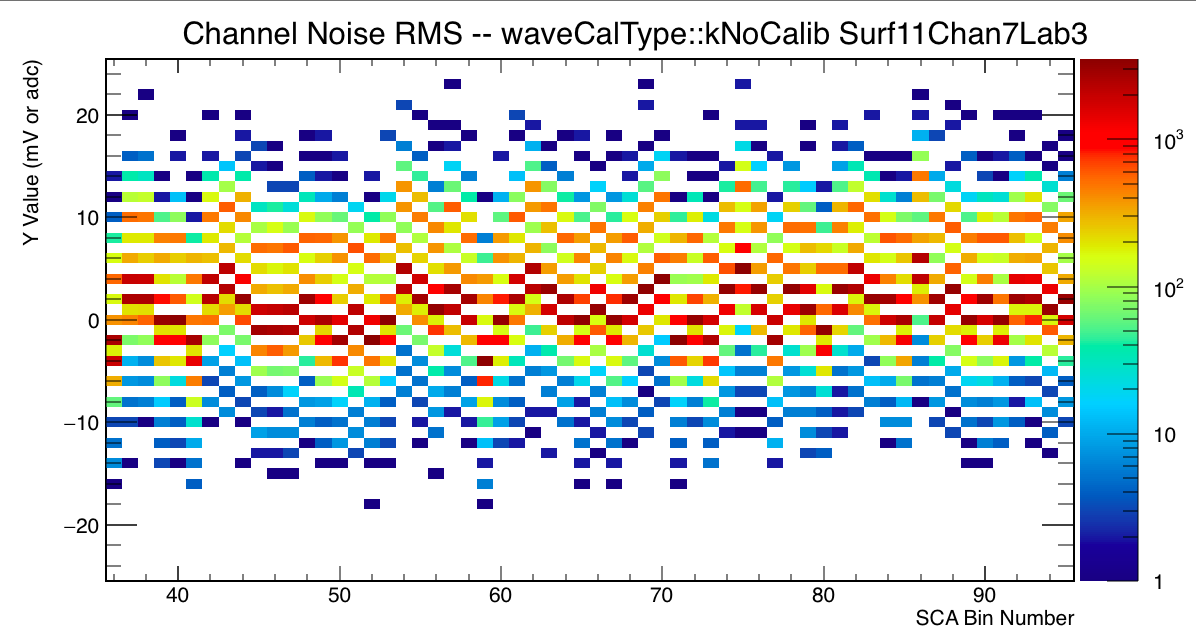
\includegraphics[width=\textwidth]{figures/pedsEvenOdd}
		\caption{A histogram of ADC count occupancy as a function of capacitor bin stored by the acquisition software.  The least significant bit from the LABRADOR is masked to zero, however the constant pedestal subtraction has a LSB addition that causes an offset.}
		\label{fig:evenOddPeds}
	\end{figure}
		
	
	
	\subsubsection{Simple Voltage to ADC Count Calibration}
	To initially measure the scaling between voltage and ADC counts of the LABRADOR chips, an identical RF pulse was inserted into two preamplifier channels, then measured both after the full signal chain immediately before entering the SURF RF input with a calibrated Tektronix oscilloscope, and again from the LABs using the ANITA readout software.  The calibration set up is shown in Figure \ref{fig:calSetup}, note that this figure is used in multiple calibration analyses.  The peak to peak height of the measured signal from the LAB chips was then compared against the pulse read out by the acquisition software and used to determine a scaling on a chip to chip basis.  While keeping the reference channel constant, the test signal was moved throughout the remaining 95 channels.
		
			
	\begin{figure}
		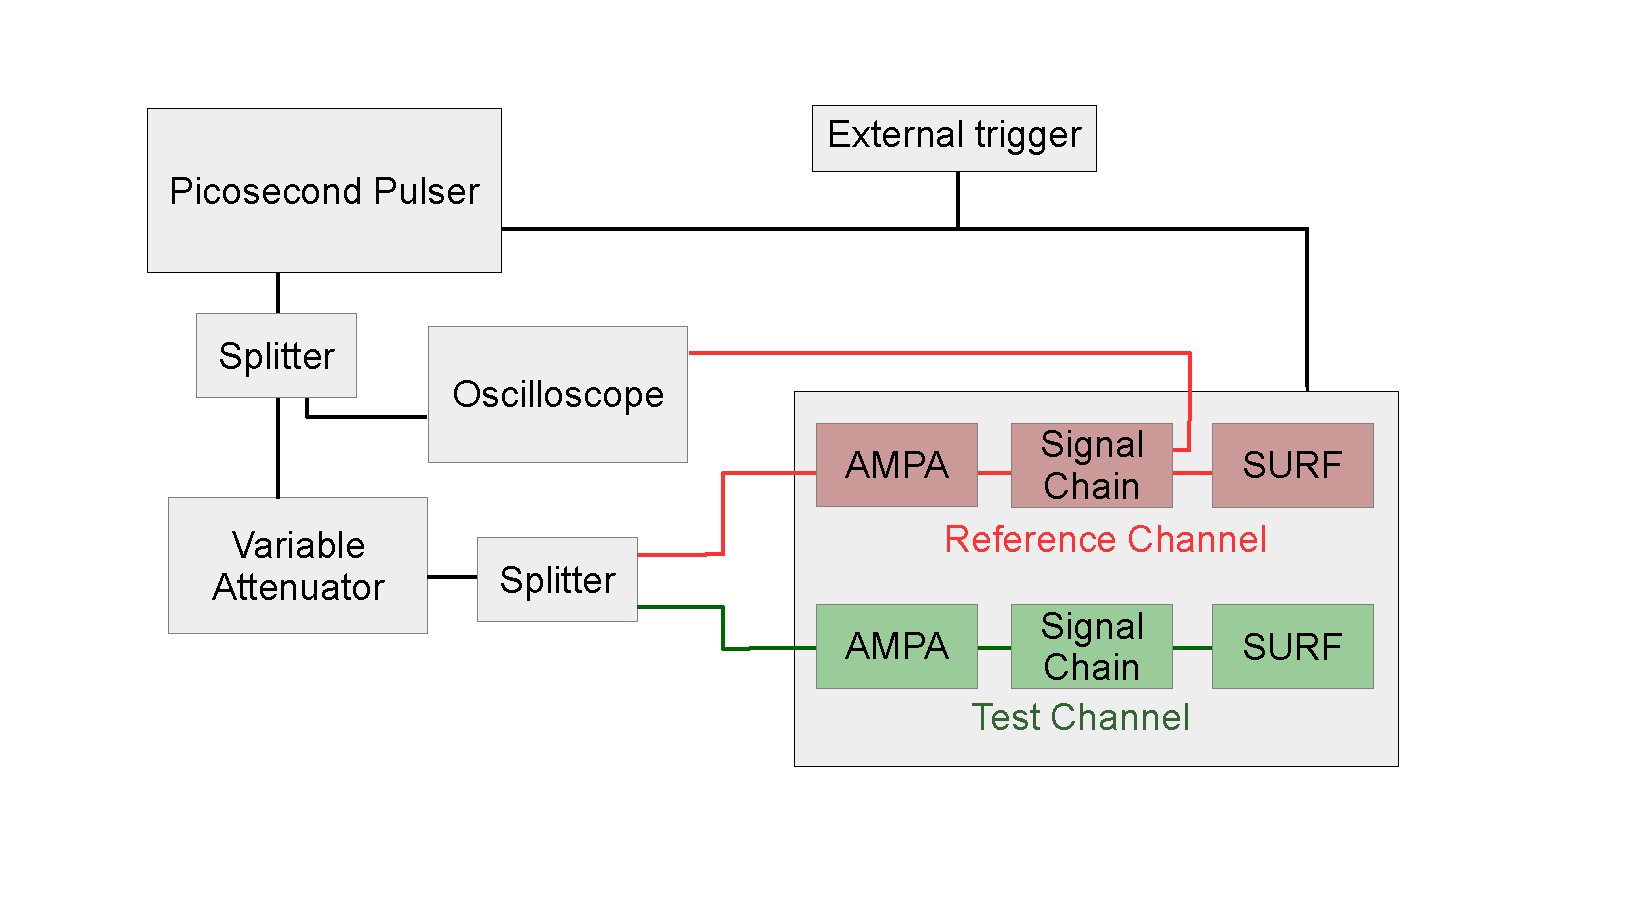
\includegraphics[width=\textwidth]{figures/antarctica14_calSetup}
		\caption{A schematic of the pulse insertion calibration setup used immediately before flight with the full signal chain in Antarctica in 2014}
		\label{fig:calSetup}
	\end{figure}
		
	One drawback of this method is that only the reference channel is coupled out from after the signal chain for comparison with the SURF output pulse.  This pulse is dispersed by the amplification and filtering of the signal chain, and thus comparing it to the input pulse requires the full complex impulse response, which considers both gain and phase as a function of frequency of the system, an analysis that is described later in this chapter.  For a simple first-order voltage calibration, one assuming voltage to be a linear function of ADC counts with no frequency dependance and an identical complex impulse response between signal chains, the peak to peak amplitude of each test channel compared to the reference channel is sufficient.  However, since the magnitudes of the gains of the signal chains is not equal, this calibration serves best as a normalization between the full signal chains of all the channels.  In other words, after applying the simple volts to ADC counts calibration, all channels are expected to have equal peak to peak voltages for an identical input signal regardless of signal chain gain or noise figure.
		
	The ADC counts to mV conversion resulting from this analysis can be seen in Figure \ref{fig:adcTomV}.

			
	\begin{figure}
		\centering
		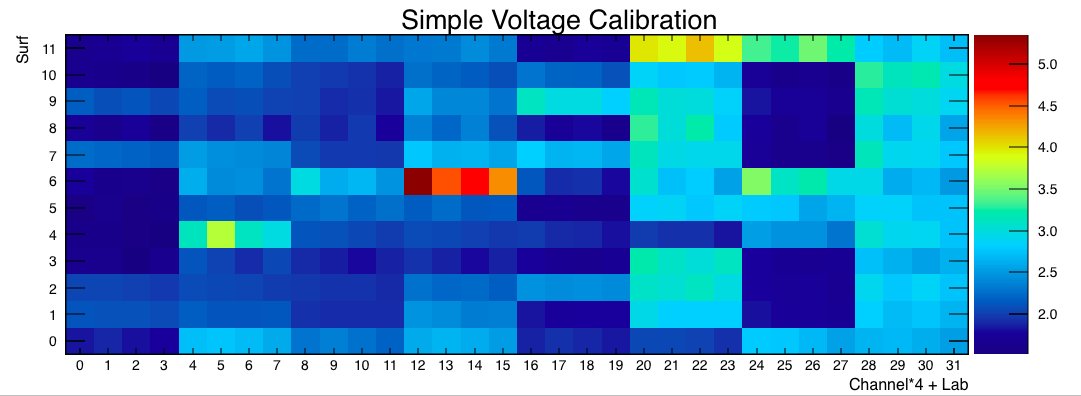
\includegraphics[width=\textwidth]{figures/ADCtoVolts.png}
		\caption{Simple voltage calibration values for all 96 channels of the ANITAIII instrument (taken from simpleVoltageCalibrationHarm.txt).  The units of the Z-axis color bar are in mV/ADC counts.  Note that each channel is digitized by four separate LAB chips.  However, the largest effect on the voltage calibration is from variations in the signal chain}
		\label{fig:adcTomV}
	\end{figure}
		



\section{LABRADOR timing calibration}
		The LAB3 storage capacitors' time base are controlled by a series of current starved transistors propagating a pulse down the array.  This pulse runs continuously and asynchronously to the global digital clock.  The pulse is also output to the FPGA as a diagnostic logic signal called the Ripple Carry Out (RCO).  This circuit allows each capacitor cell to be periodically and sequentially connected to the input signal for a fixed time interval before being disconnected, leaving a stored charge on each capacitor related to the voltage at the sampling time which can then be later digitized.  While the capacitor is connected to the input signal, it is referred to as being in ``tracking mode''.  This timing generator circuit is effected by process parameter spread in the ASIC manufacturing process, and thus does not create equally spaced time separations between capacitors in the sampling array.  The timing separation, or delta-times (dTs for short), of each sample is shared between all eight channels of each LAB chip, since it is generated by the same timing generator, however it can have significant variance between the different chips within a single SURF as well as between the SURFs.  There are 96 total lab chips actively recording data in the ANITAIII instrument, and each must be calibrated for this dT variance.

\noindent		
\begin{figure}
	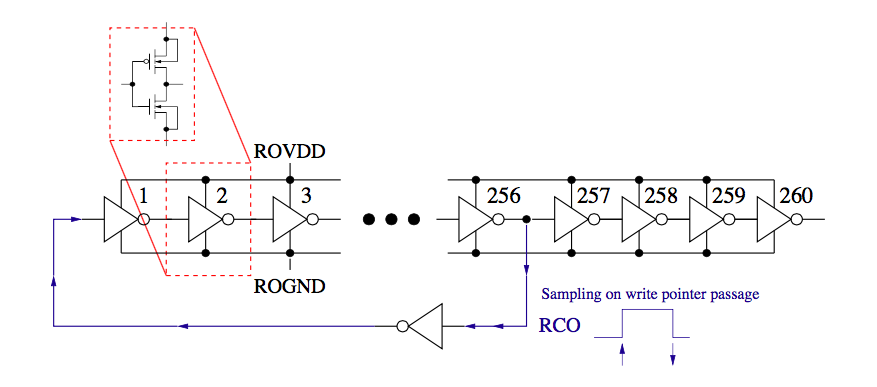
\includegraphics[width=\textwidth]{figures/LAB3BTimingGenerator}
	\caption{Diagram of LAB3B timing generator circuit\cite{LABASICPAPER} }
	\label{fig:timingGenerator}
\end{figure}

	\subsection{Time Domain Bin Width Matrix}
		The time bin width calibration constants, dTs, must be generated for each LABRADOR chip, of which there are 48 in ANITAIII, for each of the 260 samples per chip, as well as for each phase of the write strobe (up-going or down-going), leaving us with 520 total calibration constants per LAB and 24960 total values. There are several methods that can be utilized to determine the timing separation between any two capacitor bins, three of which were used to check the calibration of the ANITAIII instrument.
		
	\subsubsection{Bin Occupancy Fraction Method}
		
		The first calibration technique I will refer to as the Bin Occupancy Fraction method.  This method involves injecting a constant periodic signal, either a digital clock or a constant frequency sine wave, into each of the LAB chips.  By recording a large number of events, we can measure the resulting number of zero crossings that occur between each capacitor bin pair.  By comparing this occupancy vs the expected occupancy for a uniformly sampled time window, in which each bin observes the same number of zero crossings, it is possible to determine the fractional width of each bin.  A drawback of this method is that it requires very large statistics to reduce the uncertainty on the resulting dT.  
		
		This calibration was done for ANITAIII with two timing sources, an injected 432.1MHz sine wave and the 33.3MHz square wave sync clock injected into the system for the entire flight.  The sine wave calibration, preformed by Ben Strutt and detailed in his thesis (\cite{BenSThesis}), is the nominal calibration that is used for the remainder of this thesis.  The array can be seen in Figures \ref{fig:dTNominal2D} and \ref{fig:dTNominal2D}.  All other bin width matrix timing calibrations detailed below were done as a check on those values.
		
	\begin{figure}
		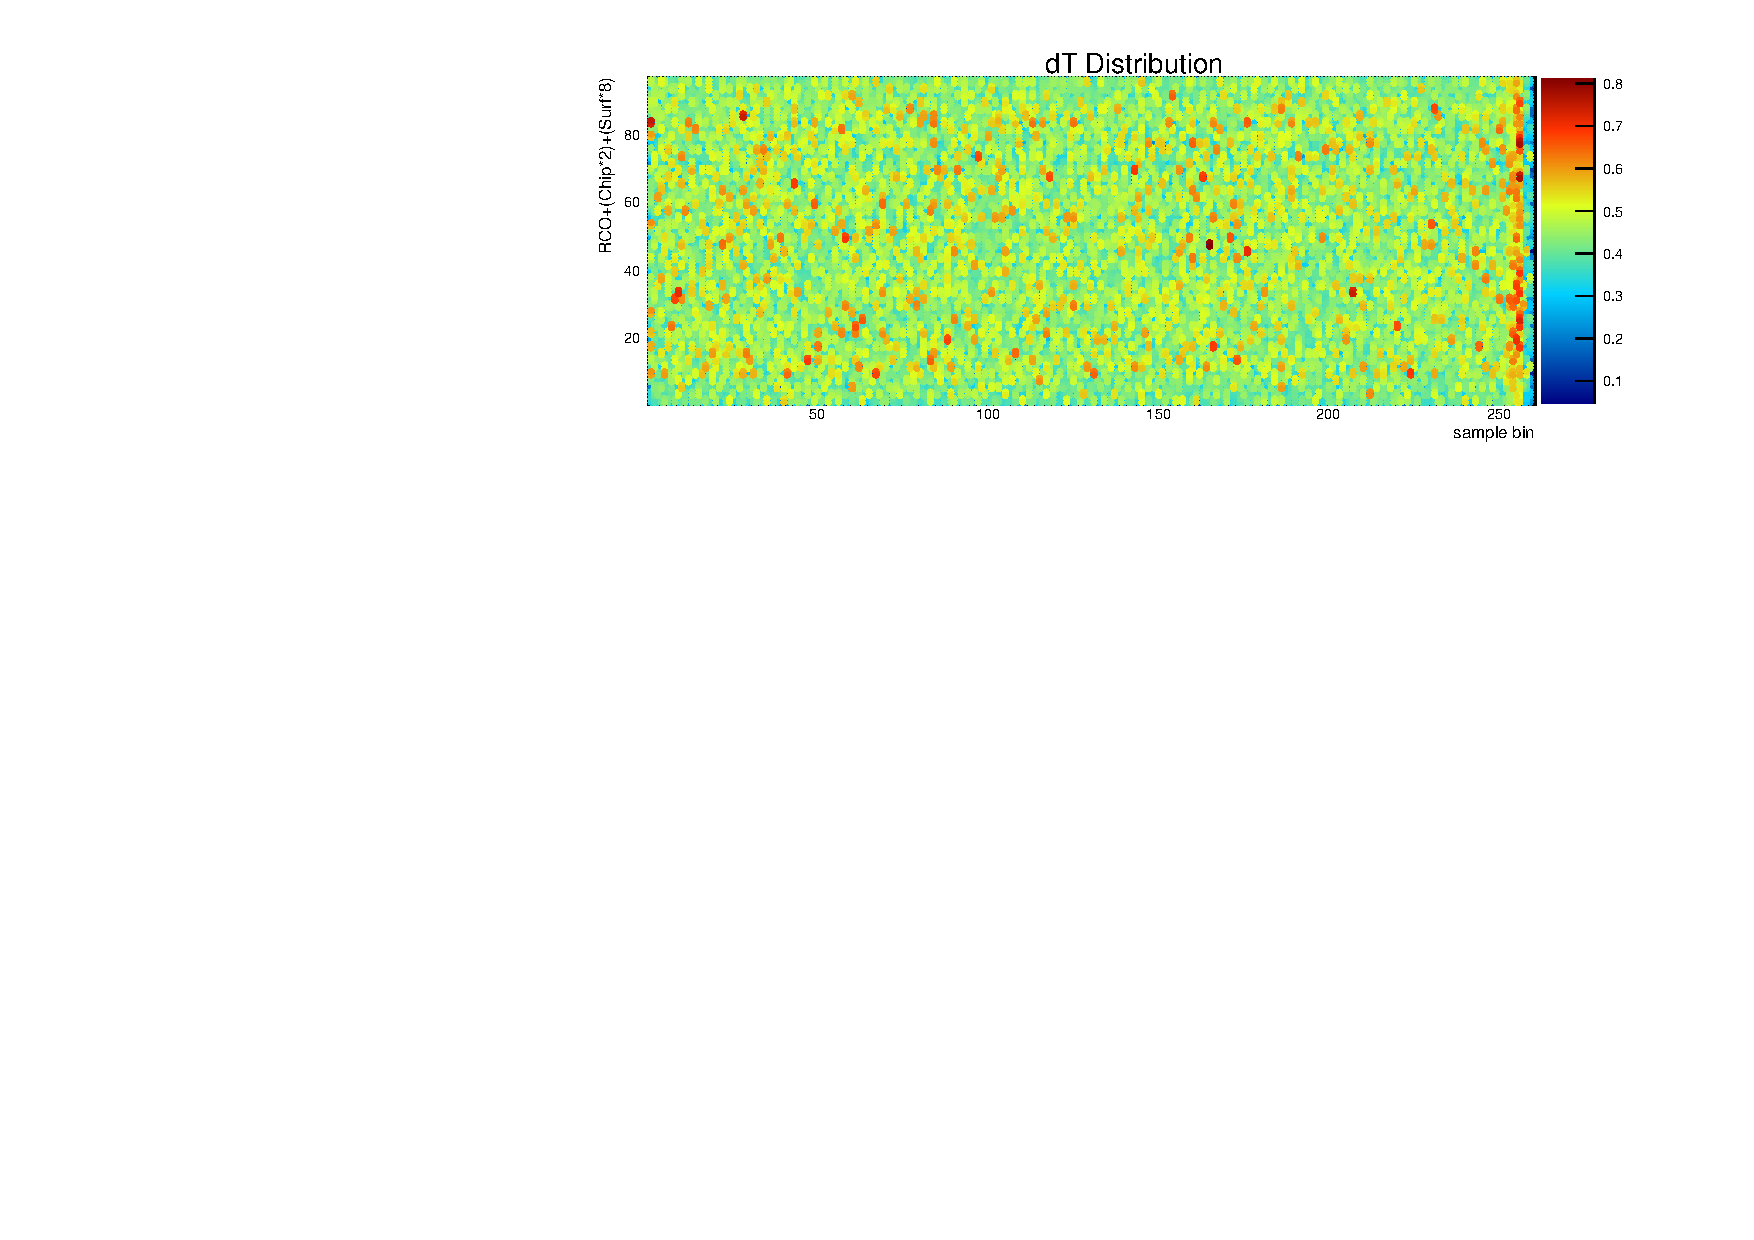
\includegraphics[width=\textwidth]{figures/dTNominal2D}
		\caption{Nominal LAB3 Time Domain Bin Width "dT" values generated using a 432.1MHz injected sine wave calibration signal and the bin occupancy fraction method.  Values were determined by Ben Strutt\cite{BenSThesis}.}
		\label{fig:dTNominal2D}
	\end{figure}
	
	
	\begin{figure}
		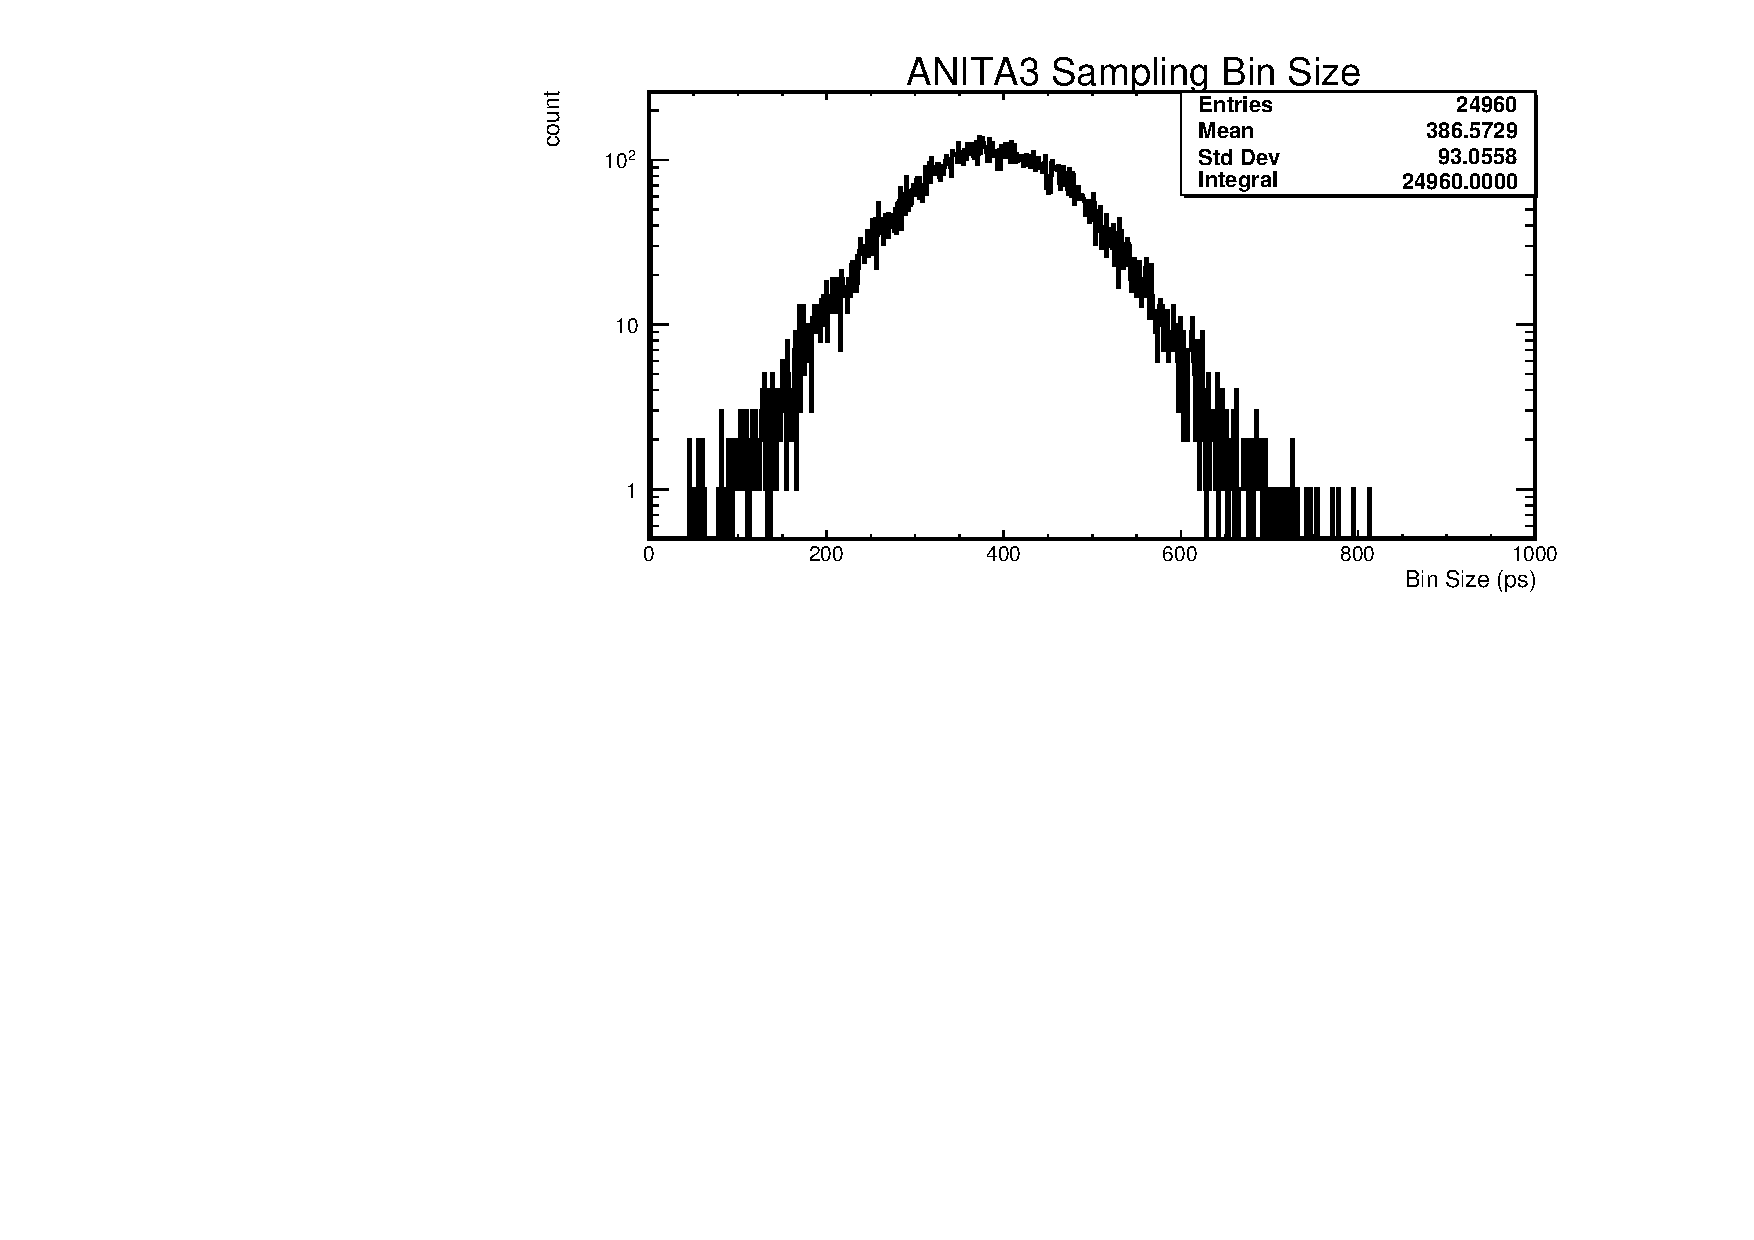
\includegraphics[width=\textwidth]{figures/dTNominal}
		\caption{Nominal LAB3 Time Domain Bin Width "dT" values generated using a 432.1MHz injected sine wave calibration signal and the bin occupancy fraction method.  Nominal values displayed in this plot and used for initial analysis were determined by Ben Strutt\cite{BenSThesis}.}
		\label{fig:dTNominal}
	\end{figure}
		
		The second possible calibration source, the 33.3MHz sync clock, is also useful for this calibration method.  Though the duty cycle of the clock has undesired variability, full period lengths are stable.  Using the falling edge of the clock provides a periodic signal with which to populate timing bins and derive their width.  It has the additional benefit of being constantly present throughout the entire flight, as well as throughout the pre-flight period in which amplifiers were off yet data was continuously being taken for stability validation.  Results of this analysis using only pre-flight runs where amplifiers were off are compared to the nominal values in Figure \ref{fig:dTNominalVsSyncClock}.
		
		
	\begin{figure}
		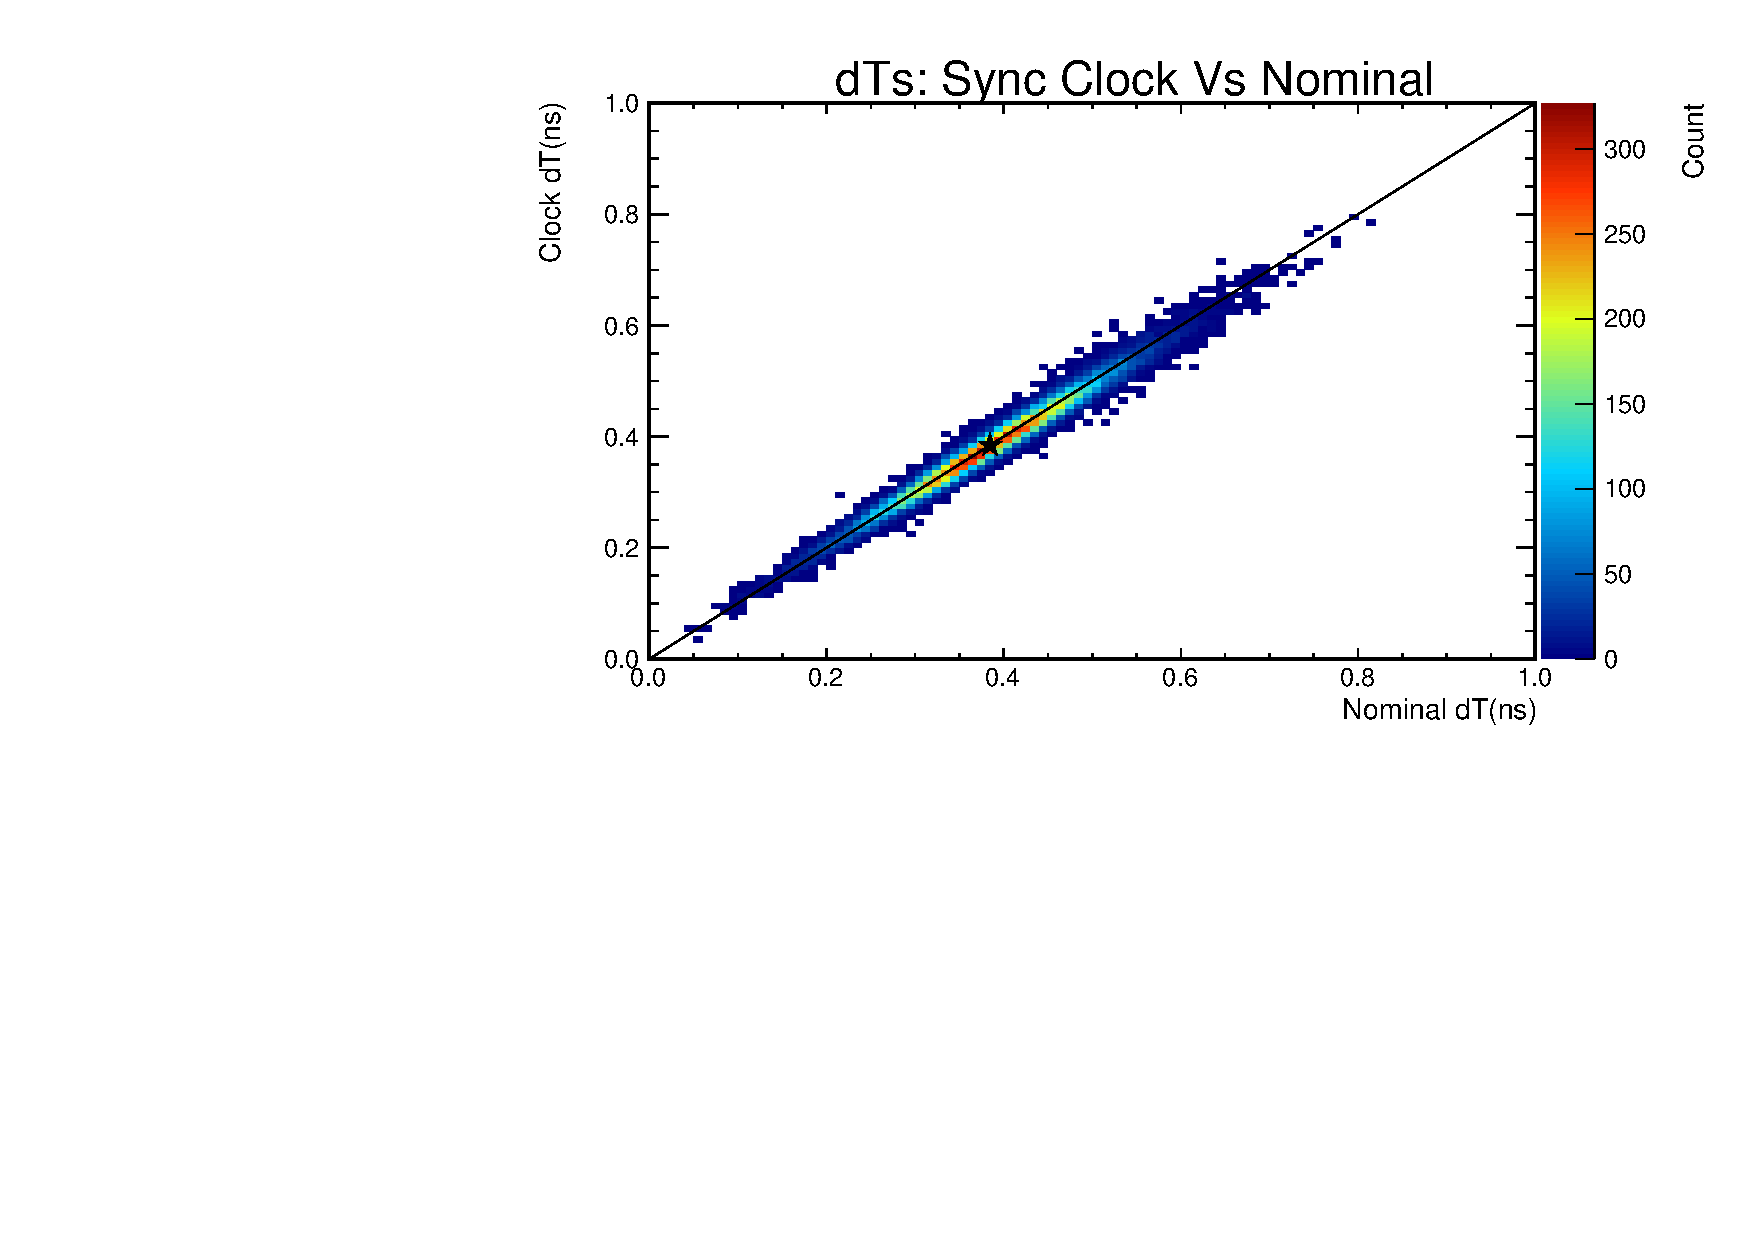
\includegraphics[width=\textwidth]{figures/nominalDtVsSyncClockDt}
		\caption{Comparisons of the derived bin widths for all channels using injected sine waves (nominal) and the 33MHz synchronization clock.  The star marks the 2.6GS/s design sampling rate, and the black line marks where the two derived values would be identical.}
		\label{fig:dTNominalVsSyncClock}
	\end{figure}


	\subsubsection{Ellipse Method}	
		The second calibration technique is slightly more clever, and involves utilyzing a characteristic of a significant number of phase offset sine waves captures and will be called the Ellipse method.  Plotting the sum and difference of sequential samples of a pure sinusoidal function yields an ellipse whose semi-major and semi-minor axes determine the fractional time of each sample.  
		
		Using this method, whose derivation is detailed in Appendix B, it is possible to determine the width of each bin by comparing the sum and difference of digitized values from neighboring bins that are offset by some time $\delta t$ both observing the same sine wave.  It is useful to consider the edge cases of such a system, for example two bins that have a negligible dT separation.  In this case the measured voltage difference between them will always be small if not zero, while the addition axis has a can a large range of values, the maximum being the crests of a sine wave. This will yield an ellipse with a very large eccentricity.  Inversely will have the inverse eccentricity, bins that are separated by exactly one half wavelength of the injected frequency will always have wide range of possible differences, and sums always approaching zero.  Nominal sampling between these extremes will provide an ellipse approaching a circle, as seen in Figure \ref{fig:ellipseMethodExample}.  This method is useful in that it requires far less data than the Bin Occupancy Fraction method.  
		
		Utilyzing this method, I calibrated all capacitor bin dTs and compared the results with the previously measured constants provided in this thesis and other published results\cite{BenSThesis}.  The values are presented in Figure \ref{fig:ellipseResults}.
		
	\begin{figure}
		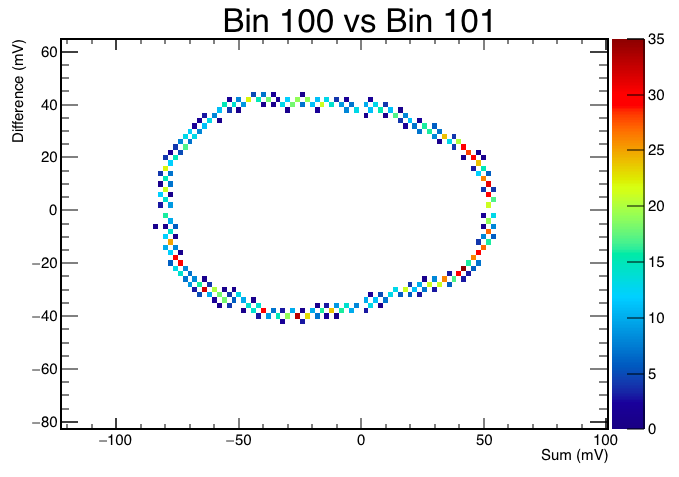
\includegraphics[width=\textwidth]{figures/ellipseMethodExample}
		\caption{}
		\label{fig:ellipseMethodExample}
	\end{figure}

	\begin{figure}
		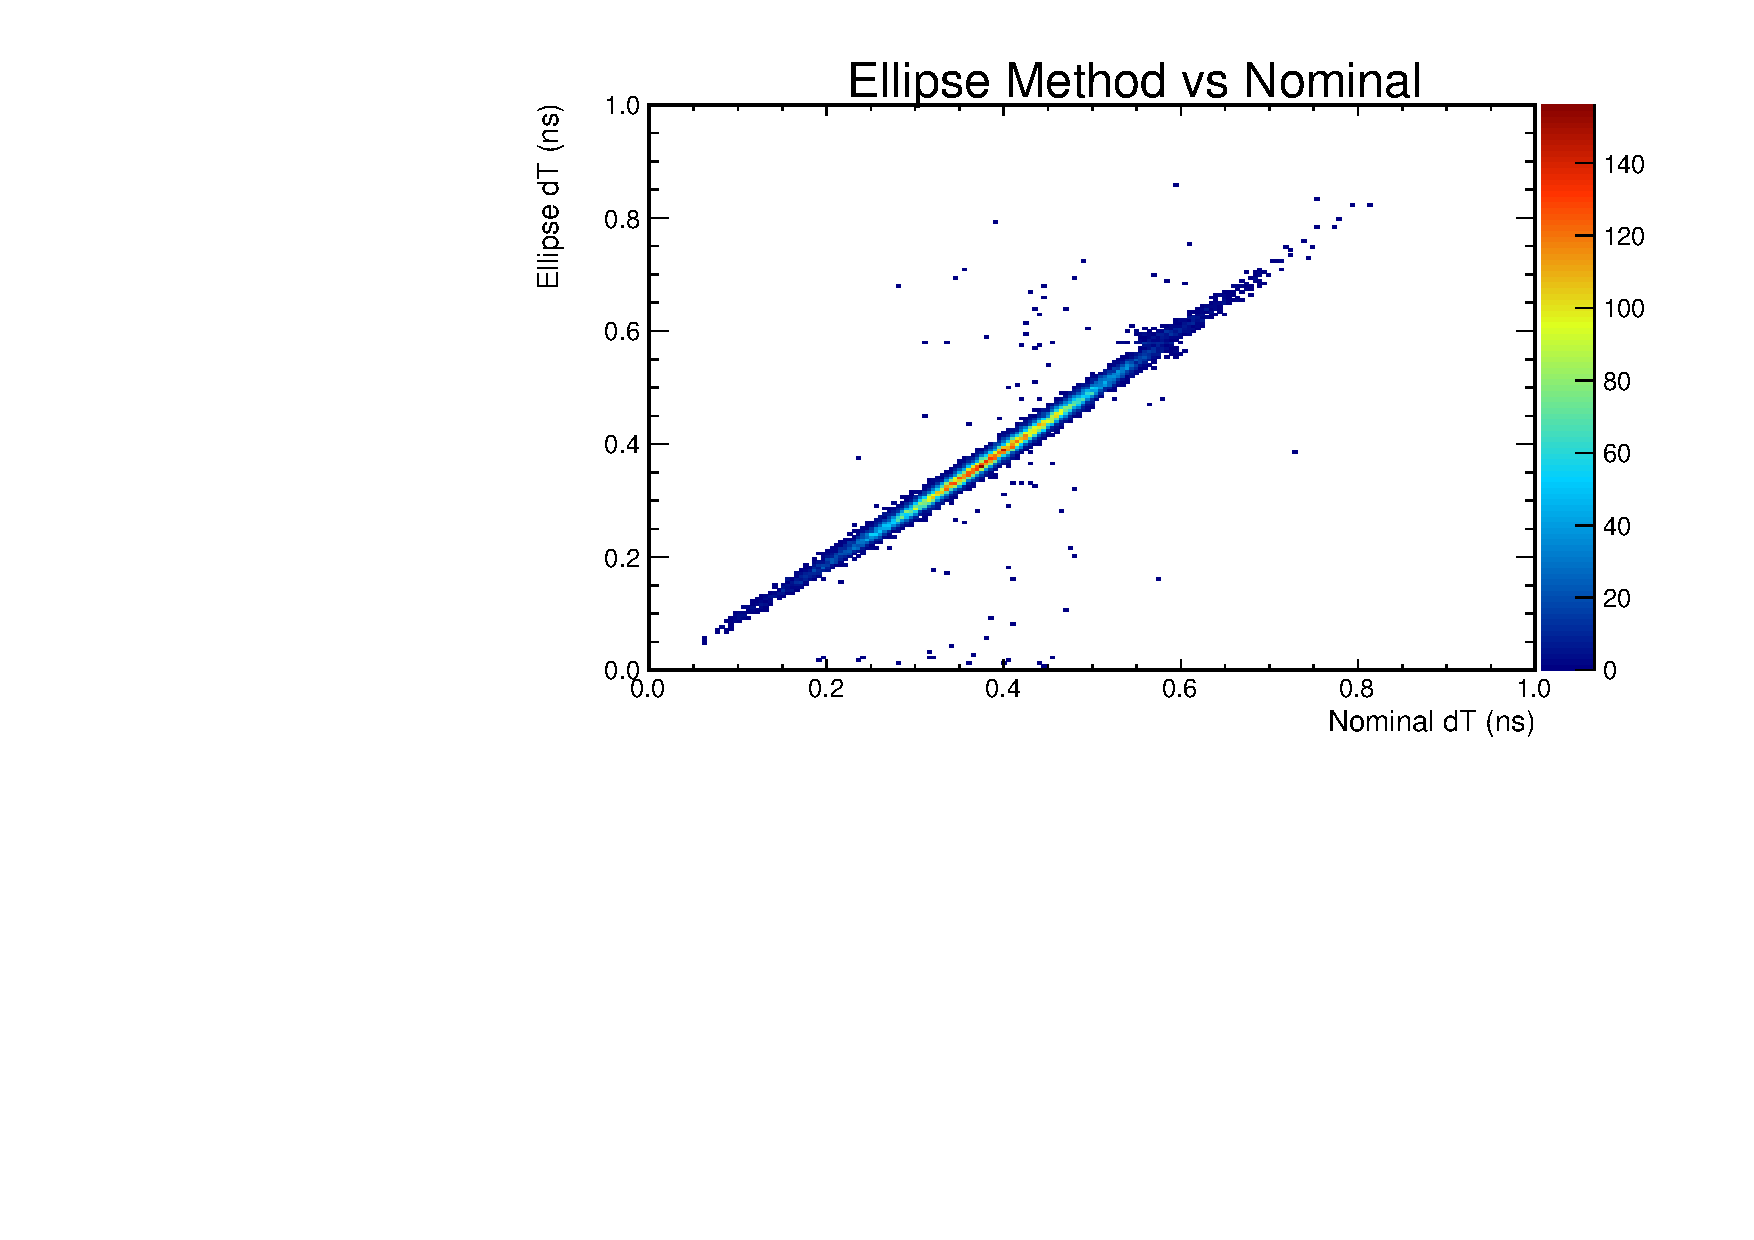
\includegraphics[width=\textwidth]{figures/ellipseComparison}
		\caption{}
		\label{fig:ellipseResults}
	\end{figure}


	\subsection{Sine Wave Fitting Method}
	
	There exists a third method for calibrating each digitizer bin's timing width, which is applying an iterative least-squares fit of the inserted sine wave and determining the relative phase offsets of the voltage of each recorded point versus the same value of the fit.  This was done as an additional method for determining the validity and event to event stability of the dT constants.  This method has the additional benefit of requiring extremely low statistics, with a measurement of the width possible on a single captured waveform.  Of course, the four LAB buffer and dual RCO phases results in each bin only being measured one eighth of the total event read out.  Additionally, the only periodic input function was a sine wave which has a large fractional region where small voltage offsets effect large timing offsets, or regions where the derivative is small.  The bin occupancy fraction method is in a way a simplification of this method, using only times where the derivative is largest.  Additionally, it is noteworthy that this method is already used to determine the Epsilon wraparound time (discussed later in this chapter).
	
	
	
	


	\subsection{dT Variance and Timing Results}	
		The variance in the timing from bin to bin has a strong effect on the measured bandwidth of the system.  Due to the non-periodic nature of the signal, bins that are sampled too far apart will be unable to digitize frequencies that are higher than the Nyquist frequency of the pair.  Similarly, samples spaced closer together than the nominal sampling frequency will act to alias in high frequency noise and dilute the signal.  The nominal sampling variance between the ANITAI and ANITAII flights increased by a factor of 3.5 to 25\%, which reduces the signal power in the high end of the spectrum .  The cause of this change between the ANITAII and ANITAIII flights is unknown, and was the reason for employing several different validation techniques of the measured dT width values.
		
		
	\subsection{Wraparound Time ($\epsilon$)}
		The propagation time of the write strobe between the end of the ring SCA and the beginning is larger than a single bin.  As the SCA acts as a ring buffer, and the pulse can occur at any time within the ring, the write strobe must begin its transition back to the first bin before the end of the SCA at bin 256.  The remaining four bins are then used to fill in the "wraparound" time, which has been colloquially called $\epsilon$.  These epsilon values, like the dT bin widths, are dependent on the polarity of the RCO signal, and so each chip receives two $\epsilon$ correction constants. In addition, four dT periods is often longer than the wraparound time, and as such the 260th sample is often treated as a duplicate and discarded.
		
		To measure these wraparound values, a sine wave is fit to the bin width corrected and unwrapped samples.  This fit is then used to derive the offsets between the last and first bins in the array.  The results of this analysis are shown in Figure \ref{fig:epsilonValues}
		
		
	\begin{figure}
		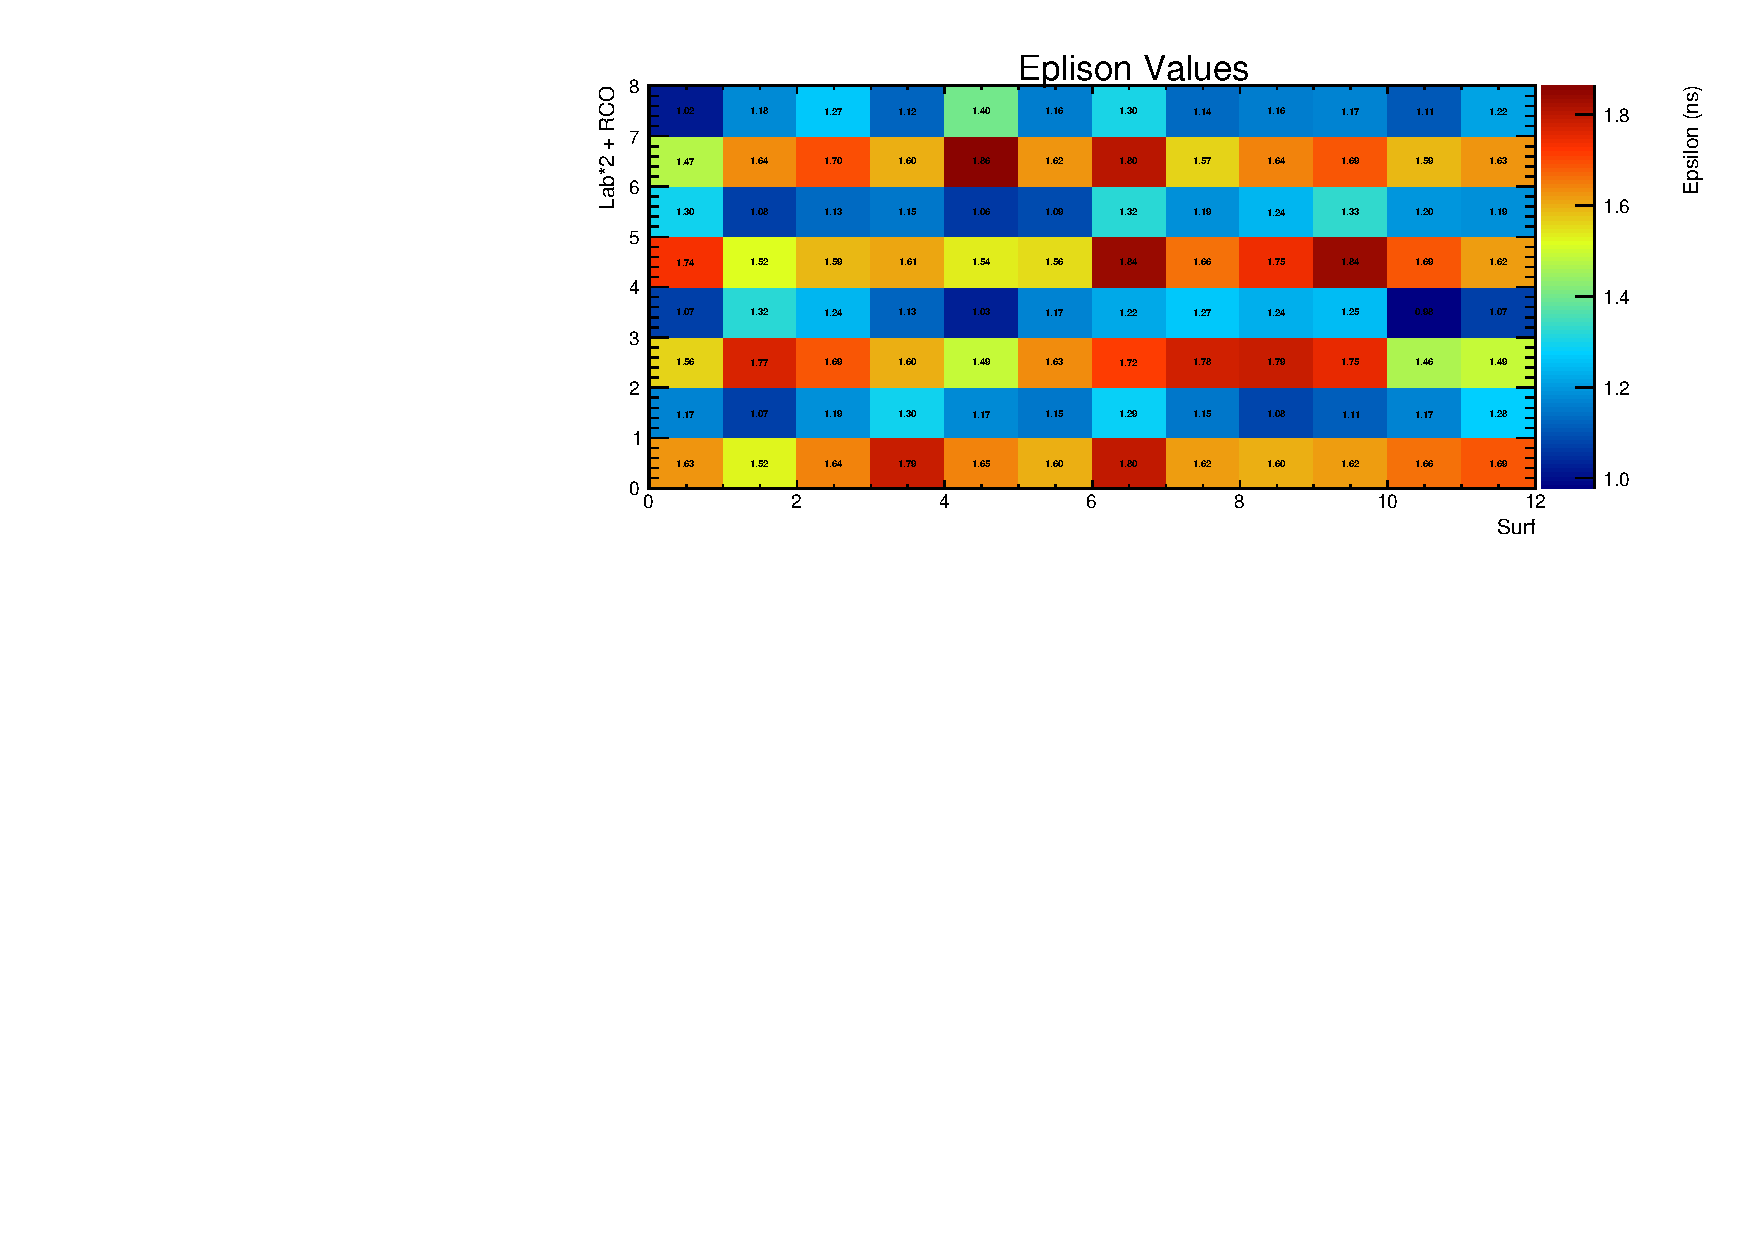
\includegraphics[width=\textwidth]{figures/epsilons}
		\caption{Measured values of the wraparound time (Epsilon) as a function of LAB and RCO phase}
		\label{fig:epsilonValues}
	\end{figure}

		
		
	\subsection{RCO Phase Determination}
		The RCO phase is sent as an output to the FPGA as a buffered copy of the wraparound voltage.  Using this, it is possible to determine the current phase of the chip when a hold was placed.  At the boundaries of the SCA, when the RCO has recently changed, the FPGA may not have the most current RCO value latched to a register when returning the digitized values.  A correction for this can be made by measuring the period of the ninth channel sync clock, which will differ between each RCO phase.  Using the firmware reported value in conjunction with the sync clock period allows for correctly determining the RCO phase with high accuracy.

	\subsection{Temperature Dependence}	
		All transistors react differently to temperature, and those present in the time base generator are no exception.  As the payload cools and warms due to rotation, time of day, and latitude, the sampling frequency will increase and decrease.  To alleviate this, a temperature correction must be applied to the final data. This is done via an average of the CP30 number reported by the FPGA over multiple events.
		

		
	\subsection{Inter-SURF Timing for Waveform Alignment}	
		As each LAB3 runs independently of each other and each channel has different signal chain group delay characteristics, each channel must be aligned in time with each other to determine the precise timing of any digitized waveforms.  The delay between channels has both a time invariant and time varying component on an event by event basis.  
		
		The invariant term, caused by the path lengths of the digitization control signals between the TURF and SURF boards in addition to any group delay offsets introduced by the signal chain, can be initially calibrated out using coincident pulses inserted into multiple channels.  To measure and correct for this offset, an impulse was sequentially injected into each channel while a coupled impulse was simultaneously injected into an unchanging reference channel.  By measuring the difference between the observed arrival times of these pulses at each SURF, it is possible to develop a matrix of constant delay offsets between channels.  This calibration setup is described in Figure \ref{fig:calSetup}.  The results of this calibration are shown in Figure \ref{fig:delayOffsets}.
		

	\begin{figure}
		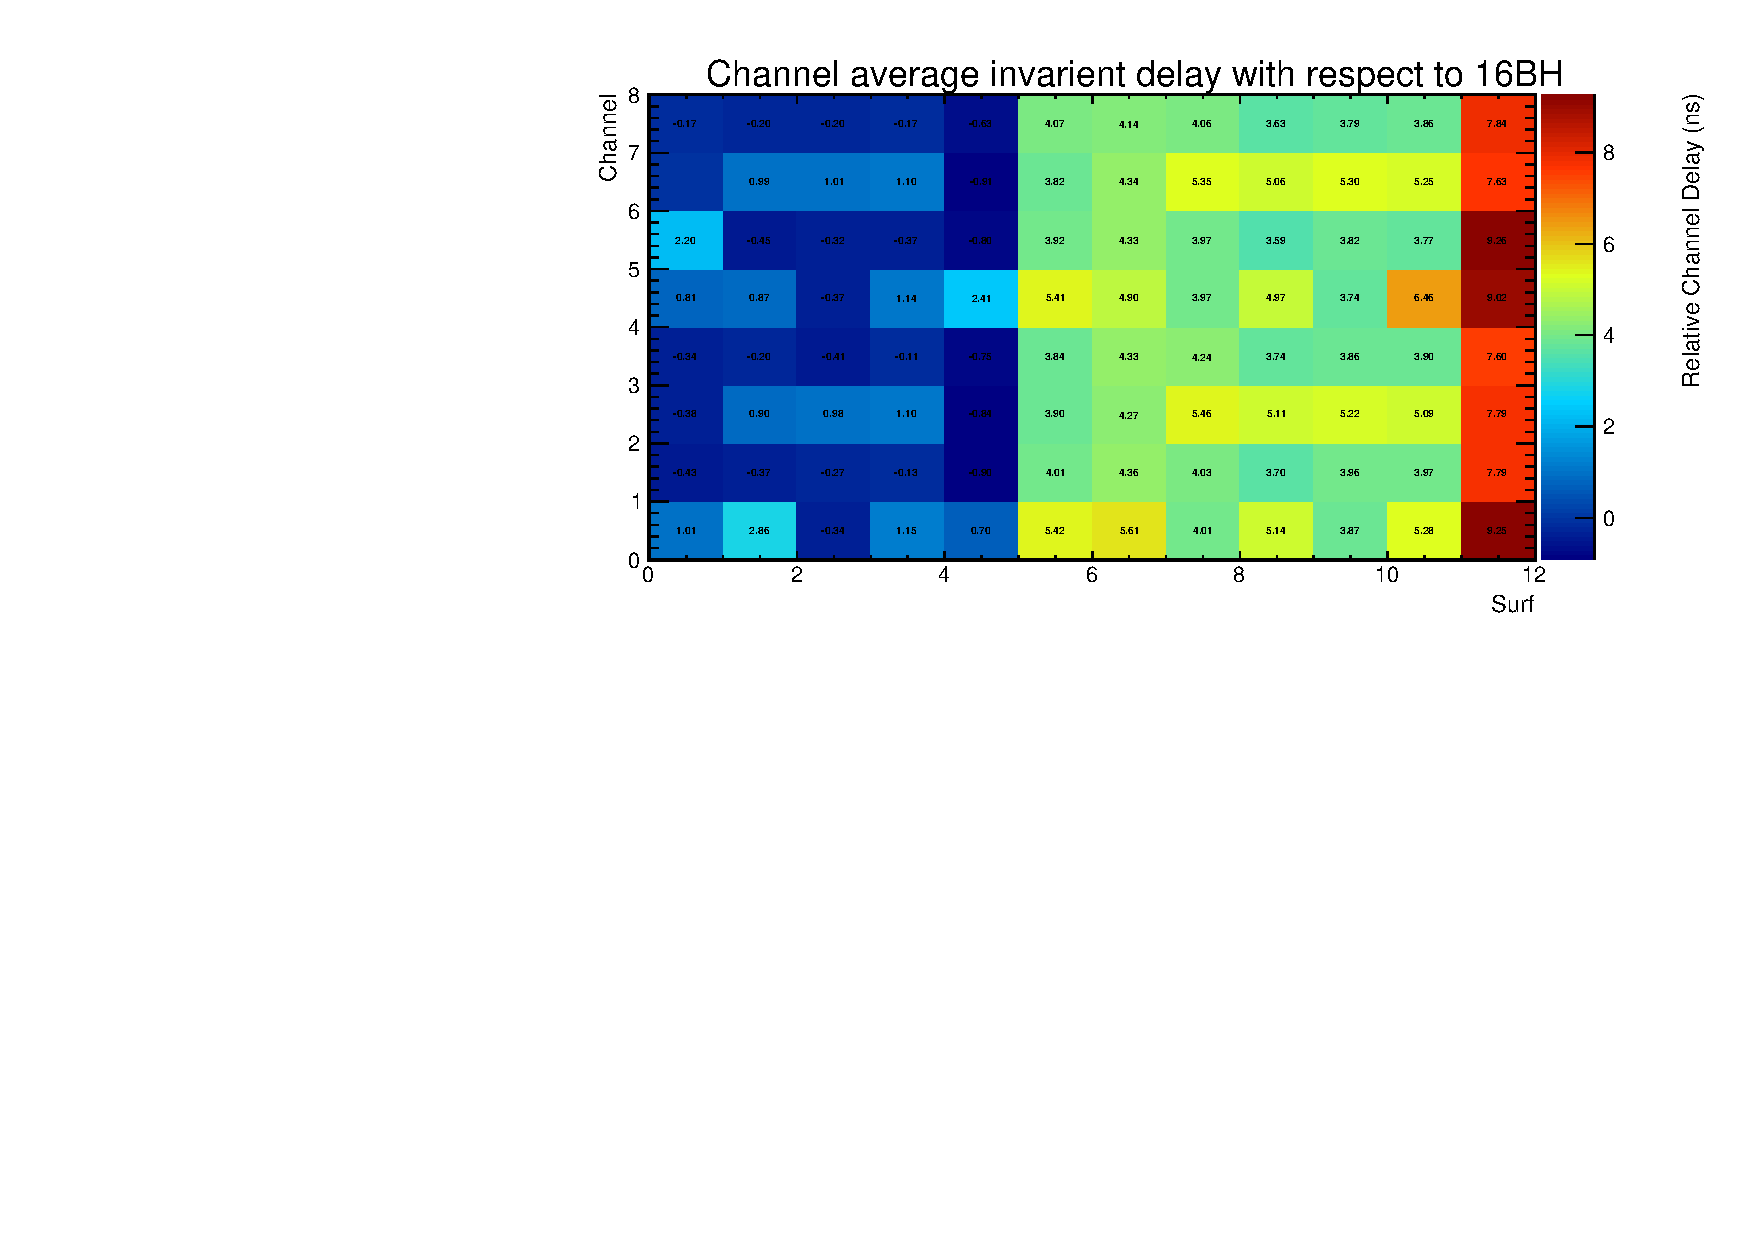
\includegraphics[width=\textwidth]{figures/averagedCableDelay}
		\caption{Channel}
		\label{fig:delayOffsets}
	\end{figure}
		
		
		The event by event time variance introduced by the nature of discrete clocked digital logic and the free-running sampling controls of the LABs, must be done at each event.  This is done with a "sync" clock that is propagated amongst the boards and constantly digitized in the 9th LAB3 channel.  This constant  33.3MHz analog clock is independent of any digital logic and thus should have a non-varying analog group delay offset between channels.  Thus, any measured offsets of the digitized sync clock between LAB channels must then be an effect of the jitter in the propagation of HOLD command and subsequent response by the LAB.  Aligning these clocks post-digitization can be used to correct for this non-varient term.
		



\section{Ground based in-flight calibration pulses}
	Three ground pulser stations, and one trailing balloon source (HiCal), were set up on the Antarctic continent for the ANITAIII flight.  These transmitted a high power, GPS synchronized, broad spectrum pulse that closely mimics an EAS impulsive radiation signature.  These pulses can be used both for determining the overall sensitivity and efficiency of the trigger system, but can also be used as known-source measurements for doing precise in flight antenna phase center location calibrations.
	
	Two autonomous pulser stations were deployed at field camps in east Antarctica, and an additional manned pulser pulser was deployed at the launch site, also known as the Long Duration Balloon (LDB) facility.  The remote stations were located at WAIS Divide and Siple Dome, however the payload only passed within line of cite of the WAIS divide pulser location.  They employed an azimuthally symmetric, quad-slot "Mini-ALFA" antenna custom designed by A. Romero-Wolf for horizontally polarized signals, and a Telewave ANT280S discone antenna for vertically polarized signals.  These are shown in figure \ref{fig:waisPulserAntenna}.  Their S11, a measure of antenna efficiency, is seen in Figure \ref{fig:waisPulserAntennaResponse}. 
	
	\begin{figure}
		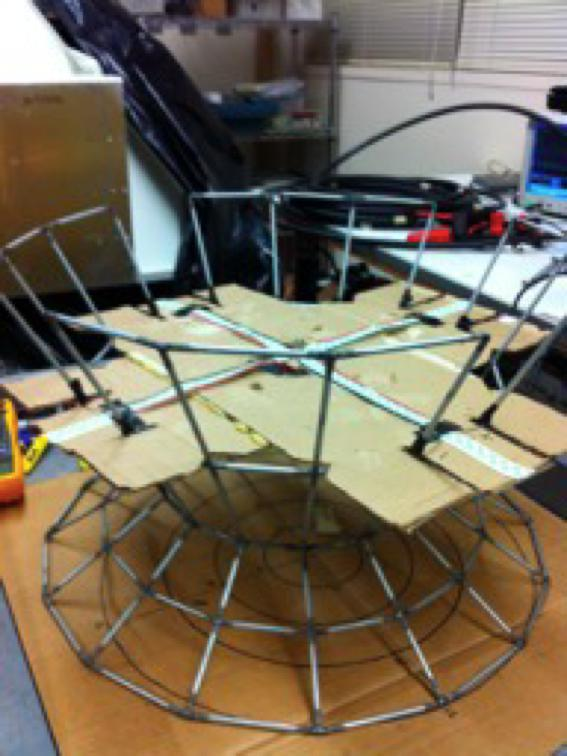
\includegraphics[width=0.45\textwidth]{figures/waisPulserAntennaH}
		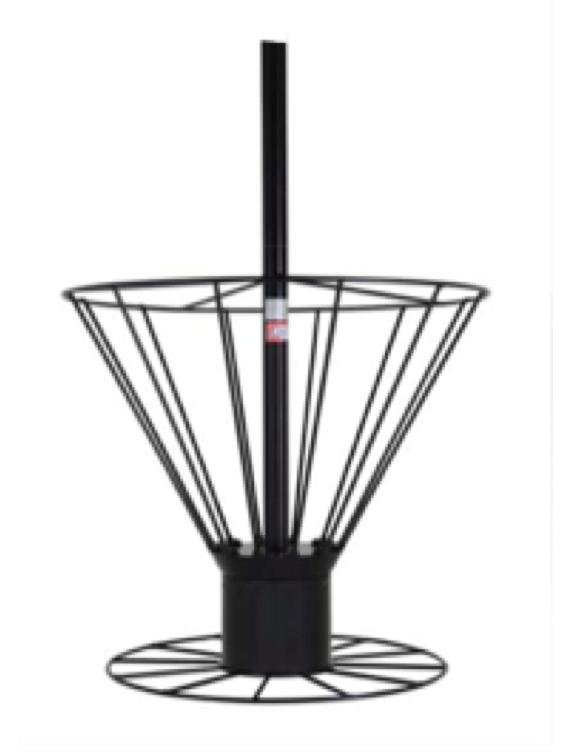
\includegraphics[width=0.45\textwidth]{figures/waisPulserAntennaV}
		\caption{Images of the calibration pulser antennas deployed at WAIS divide and Siple Dome for calibration of the ANITAIII instrument in flight.  Right: Custom designed, quad-slot "Mini-ALFA" antenna for horizontally polarized signals.  Left: a Telewave ANT280S discone vertically polarized antenna. \cite{StephCalPulserPresentation}}
		\label{fig:waisPulserAntenna}
	\end{figure}	
	
	\begin{figure}
		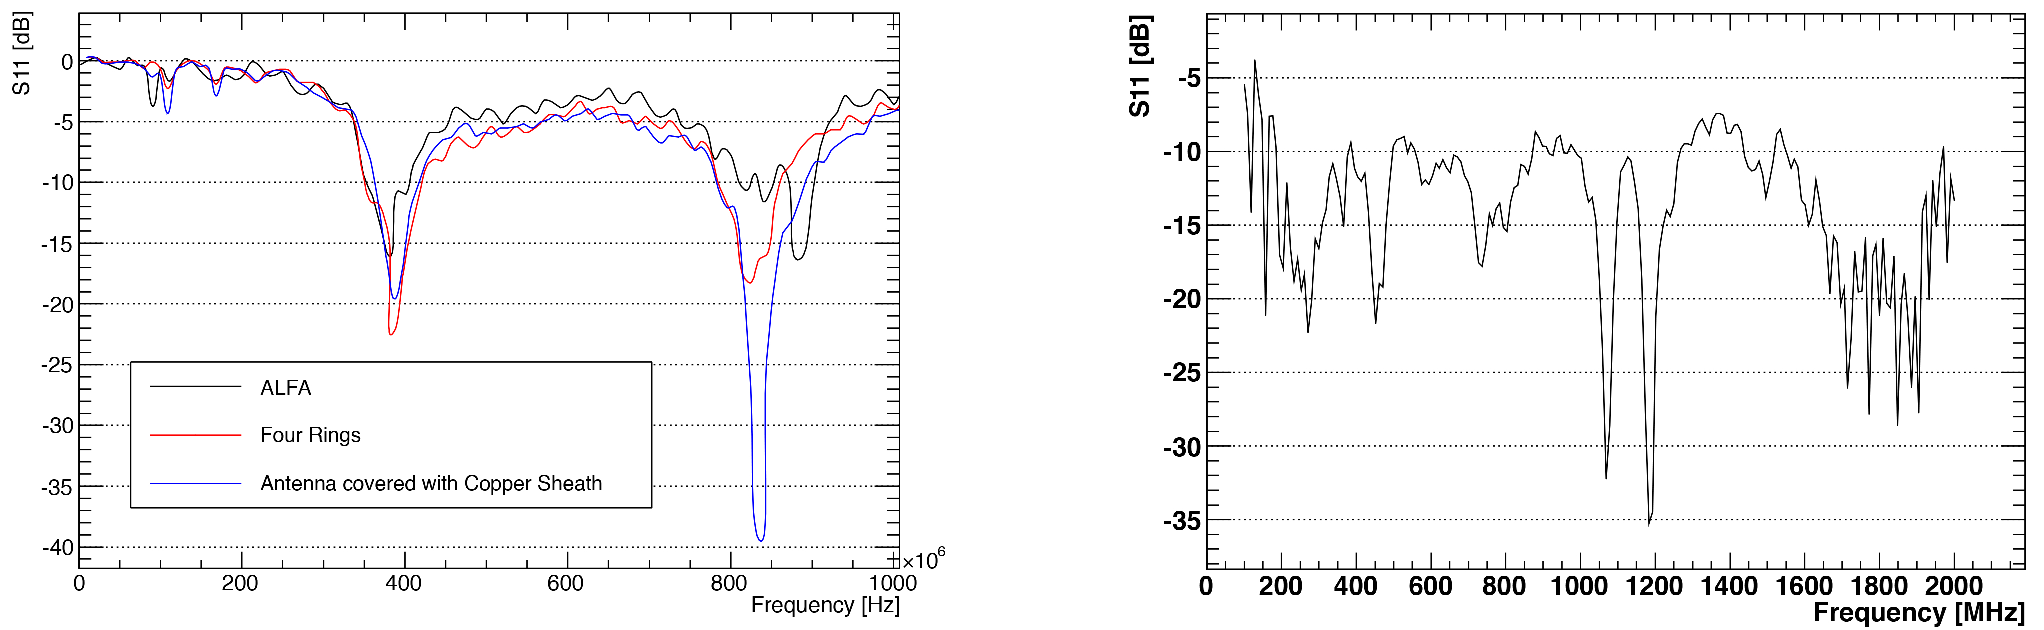
\includegraphics[width=\textwidth]{figures/waisPulserAntennaSpectrum}
		\caption{Measured S11 antenna efficiency for the horizontally (left) and vertically (right) polarized antennas deployed at remote locations for the ANITAIII in flight calibration pulsing. \cite{StephCalPulserPresentation}}
		\label{fig:waisPulserAntennaResponse}
	\end{figure}
	
	All ground based calibration pulsers and the payload timing were synchronized to the GPS second.  This was done to ensure that any calibration pulse signature could be discriminated from physics signal events easily.  The HiCal pulser system was unable to employ a GPS synchronization due to cost and weight limitations, and their existence can only be derived from the reported location telemetry from its payload.
	
	\subsection{WAIS Divide}
		The autonomous station deployed at WAIS divide consisted of two antennas, one vertically and one horizontally polarized, pulsing at a repetition rate of 1Hz.  An unknown system failure yielded only horizontally polarized pulses measured at the ANITAIII instrument.  The WAIS calibration pusles give us our best estimate for the locations of in flight antenna horizontally polarized phase centers.
		
		Discriminating between WAIS pulser events and noise or physics signal events was done by making a cut on the TriggerTimeNs quantity stored in the header section of the event data.  Since this quantity is reset on the GPS second, and the ground based calibration pulser was fired on the GPS second, the arrival time of the signal at the payload is predictable.  Figure \ref{fig:waisTrigTimeNs} shows a histogram of the occupancy of TriggerTimeNs values as a function of time.  Using the gps coordinates of both the payload and pulser to determine and correct for the time of flight and expected arrival time can be seen in Figure \ref{fig:waisTrigTimeCorr}.
		
	\begin{figure}
		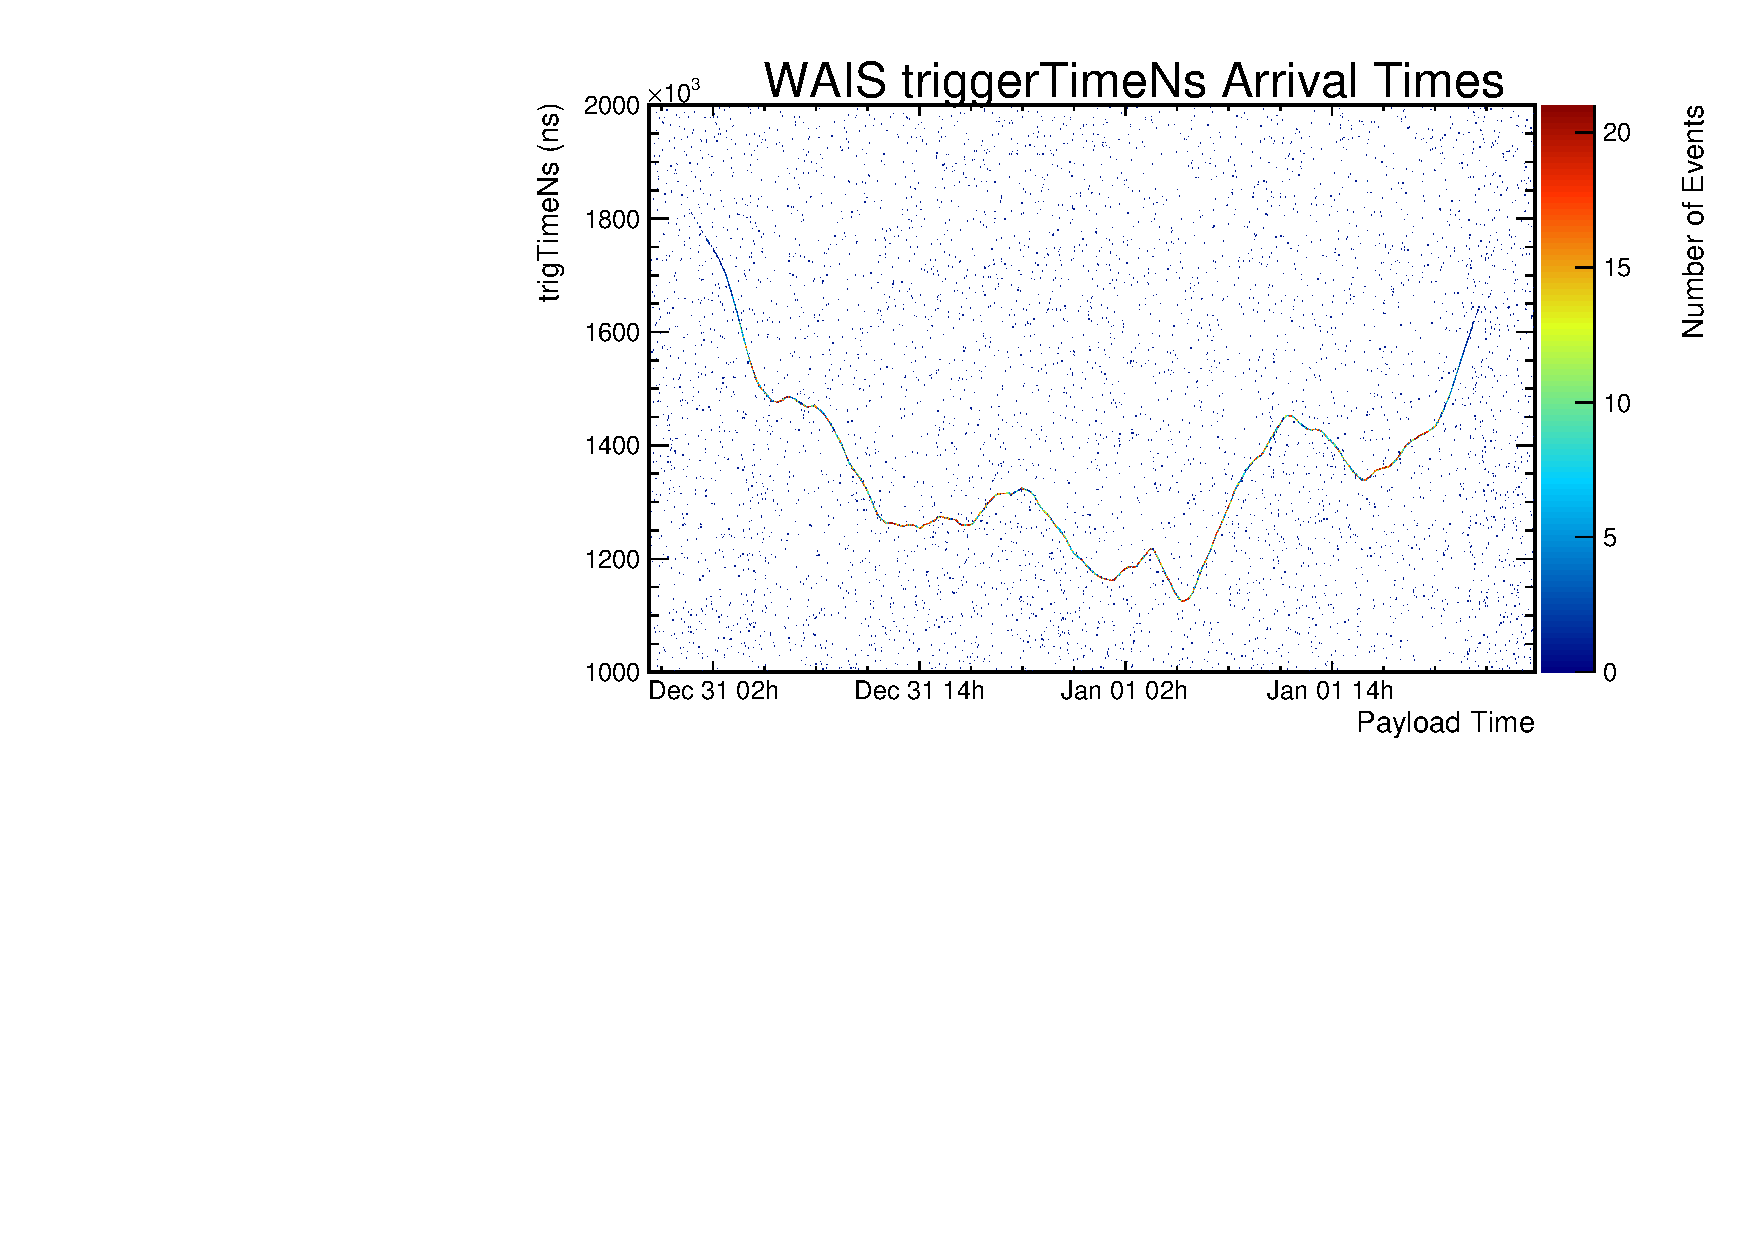
\includegraphics[width=\textwidth]{figures/waisTrigTimeNs}
		\caption{Stored triggerTimeNs trigger decision time distribution for RF triggers in the approximately two day period during which ANITAIII was within line of sight of the Wais Divide calibration pulser.  The visible line is an increase in the number of events per bin well above expectations.  The variation in the line is movement of the payload towards and away from the pulser location and the subsequent time of flight variation.}
		\label{fig:waisTrigTimeNs}
	\end{figure}		

	\begin{figure}
		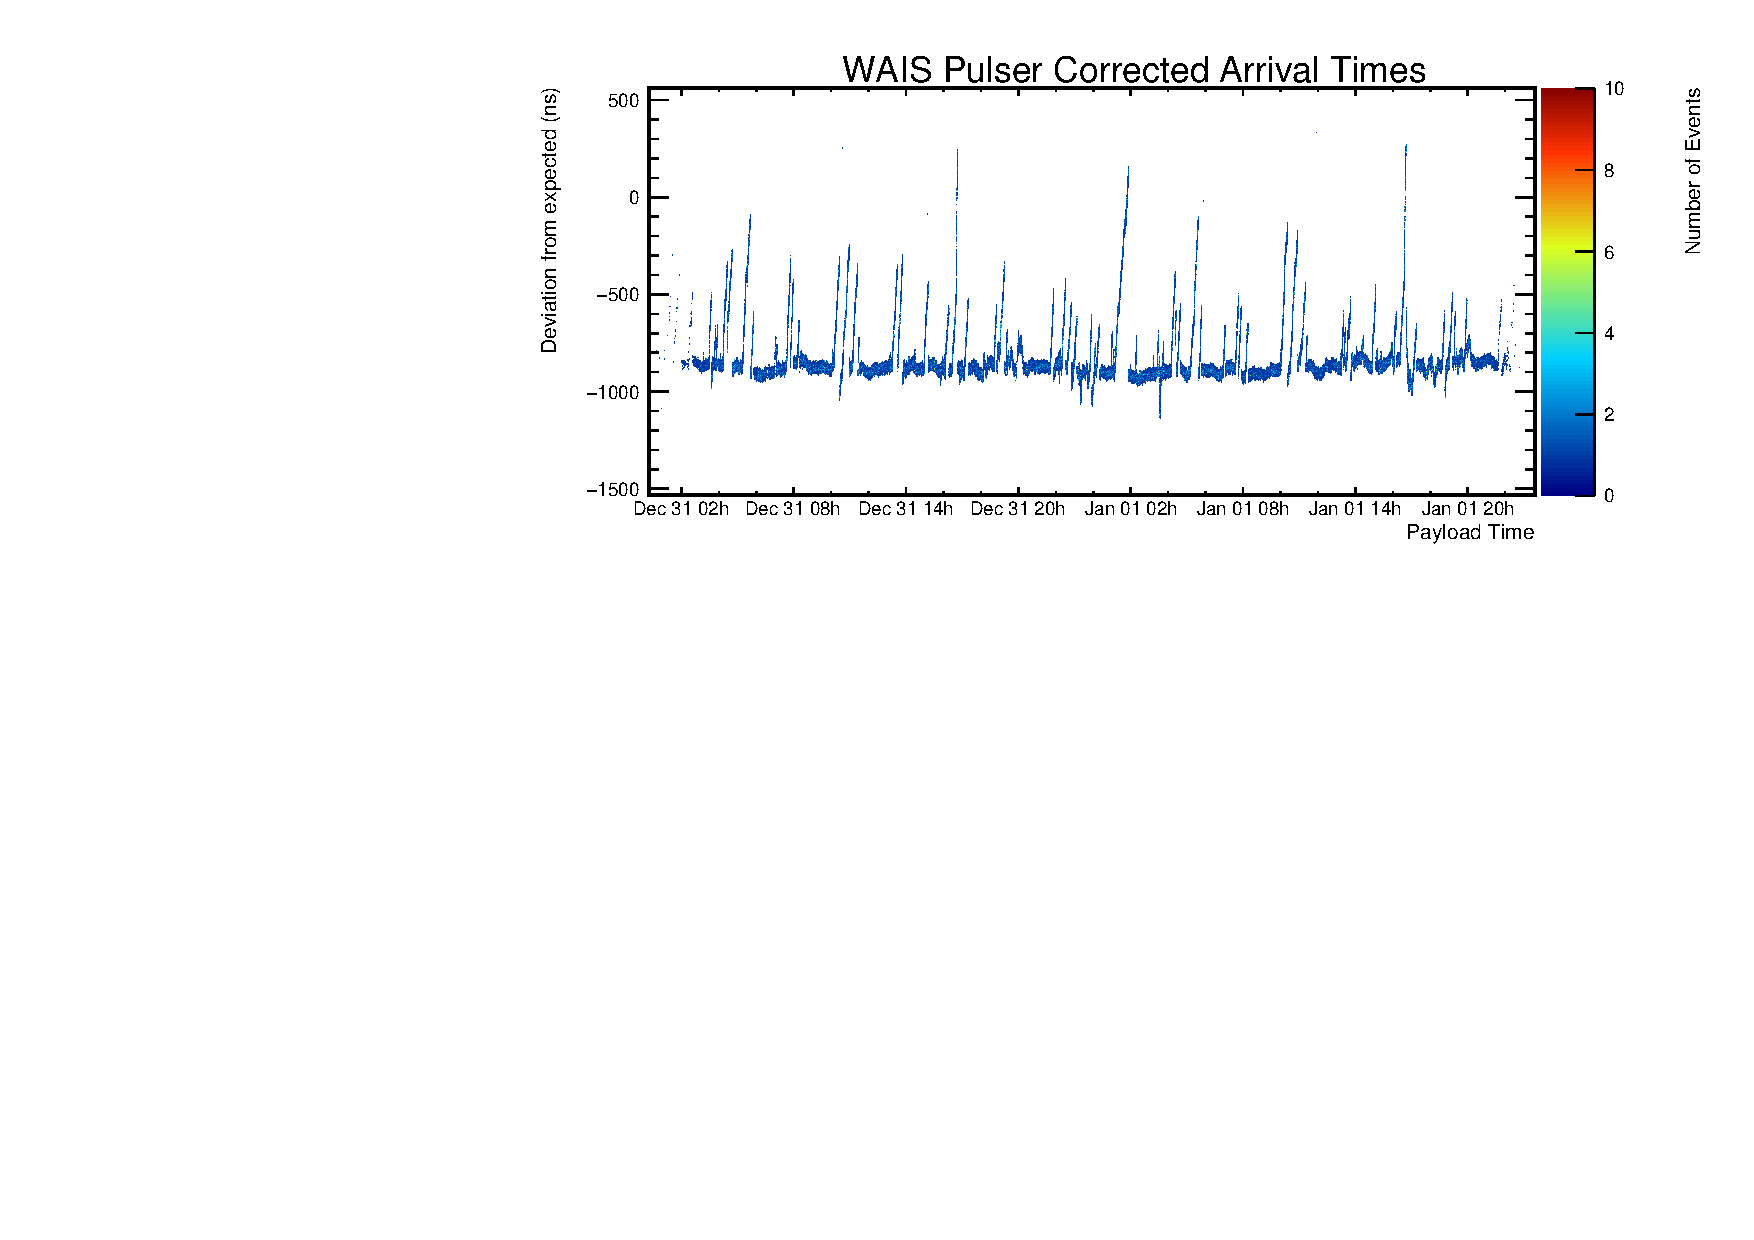
\includegraphics[width=\textwidth]{figures/waisPulserCorrNs}
		\caption{Stored triggerTimeNs trigger decision time distribution for RF triggers in the approximately two day period during which ANITAIII was within line of sight of the Wais Divide calibration pulser, corrected for time of flight to the balloon payload.  Deviation spikes from the expected arrival time, which can be seen are as large as 1$\mu$s, are likely the result of the remote pulser station losing its GPS second synchronization lock.}
		\label{fig:waisTrigTimeCorr}
	\end{figure}		
		
		

	\subsection{LDB}
		The LDB pulser was observed twice during both the initial launch period, as well as during the second pass on the subsequent orbit around the continent.  This pulser provided the only vertically polarized calibration signals.  A drawback of this pulser location is the high level of non-thermal anthropogenic noise generated by McMurdo Station and the surrounding field camps.  Subsequently, a high power level and high repetition rate of the pulser was required in order for the payload to efficiently self trigger on the signals.  Additionally, as the signals were arriving from the same direction as the noise sources, trigger phi-masking had to be turned off for these measurements, a parameter not characteristic to the majority of the flight.  Figure \ref{fig:mcmTrigTimeNs} shows the distribution of arrival times as a function of nanoseconds from the GPS PPS signal.
	
	\begin{figure}
		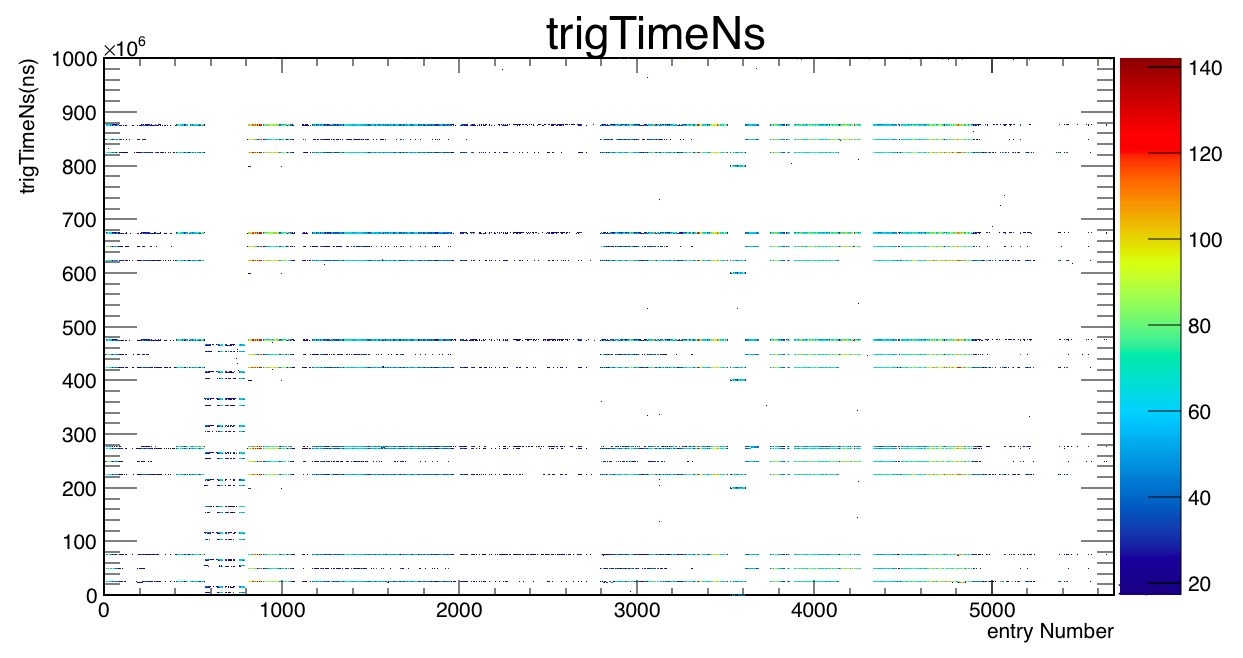
\includegraphics[width=\textwidth]{figures/mcmTrigTimeNs}
		\caption{Stored triggerTimeNs trigger decision time distribution for RF triggers immediately after launch while ANITAIII was within line of sight of the LDB calibration pulser.}
		\label{fig:mcmTrigTimeNs}
	\end{figure}		

	
%	\begin{figure}
%		\includegraphics[width=\textwidth]{figures/mcmPulserCorrNs}
%		\caption{Stored triggerTimeNs trigger decision time distribution for RF triggers immediately after launch while ANITAIII was within line of sight of the LDB calibration pulser.}
%		\label{fig:mcmTrigTimeCorr}
%	\end{figure}	
		
		
		
	\subsection{HiCal}
		As real cosmic ray EAS radiation signals are emitted in the atmosphere, it is desired to have a calibration source that mimics this source location.  HiCal utilizes a piezoelectric spark generator driven by a small DC motor attached to a horizontally polarized fat dipole antenna hanging from a balloon payload.


\section{Antenna Phase Center Location Measurements}
	To accurately reconstruct the arriving electromagnetic wavefront it is extremely important to know the positions of the antennas to very high precision.   Using Equation \ref{eqn:lightTravel} for determining the distance traversed by a travelling wave, and unscientific imperial units, a wavefront traveling at the speed of light will traverse approximately one foot per nanosecond of time. 
	
	\begin{figure}[h]
	\begin{equation}
		\Delta x = \tau c
	\end{equation}
	\label{eqn:lightTravel}
	\end{figure}
	
	The timing limitation imposed by the inter-surf timing discussed above is on the order of 10ps, which would correspond to a 3.6mm maximum uncertainty on the phase centers of the antennas before the become the limiting measurement for coherent reconstruction of several digitized waveforms.  Measuring the relative positions of these with such accuracy, or assuming their positions from a design model, is unrealistic, and so several other methods have been employed to determine their positions.
	
	\subsection{Photogrammetry}
		An initial measurement of the antenna locations with respect to each other, to the instrument box, and to the GPS antennas (and thus recorded attitude heading, and position), was done by analyzing a series of standardized photos of the payload taken from a variety of angles and rotations.  Utilyzing this data coupled with precise measurements of single antenna dimensions, it is possible to arrive at a first order estimate of the antenna positions.  An example image and subsequent wiremesh model of the payload can be seen in Figure \ref{fig:photogram1}.
		
	\begin{figure}
	\label{fig:photogram1}
		\centering
		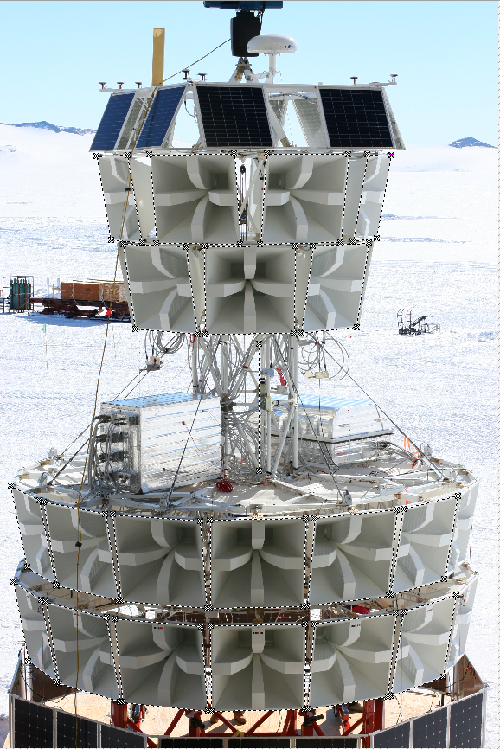
\includegraphics[height=0.5\textheight]{figures/KBelovANITA-III_photogrammetry_update-3}
		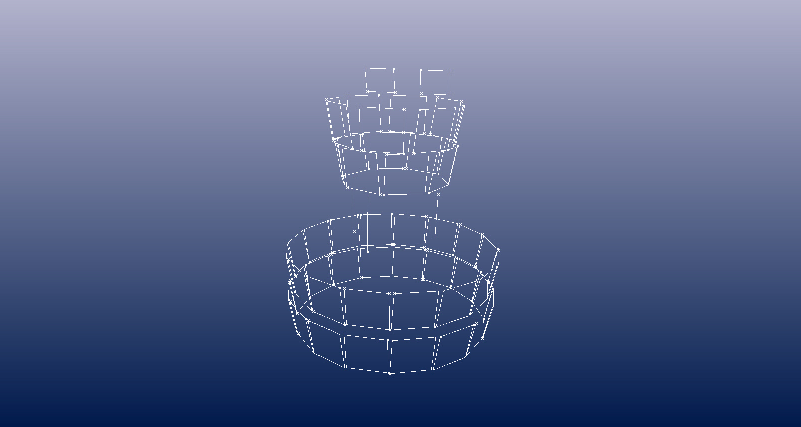
\includegraphics[width=\textwidth]{figures/KBelovANITA-III_photogrammetry_update-4}
		\caption{Top: Example photogrammetry image of the ANITAIII payload with markers drawn around the antenna face outlines.  Bottom: Subsequent wiremesh model of antenna positions derived from numerous combined images.  Thanks to Constantine for images.}
	\end{figure}
	
		
	\subsection{Calibration Pulse Timing Optimization}
		The electrical center-point of the antennas, though directly related to the physical position and orientation of the antenna, requires an additional calibration.  The phase center, or point at which the electromagnetic field couples to the antenna and begins propagating through the signal cables, is a function of frequency and incident wave direction, so the calibration must consider a large phase space.  The calibration measurements are done in-situo by a ground pulser at WAIS divide sending a pulse to the payload as it passes overhead.  This pulse can be used to determine  the relative phase center offsets between nearby antennas.  The positional error of the phase centers relates directly to the pointing error for events seen later in the flight.
		
		The two pulser locations discussed earlier provide two distinct timeframes during which to measure the phase centers of the antennas.  

\section{Instrument Impulse Response}
		The signal observed by the digitizers is strongly effected by the various components in the signal chain.  Chief amongst these is the group delay introduced by the band pass filters.  To properly reconstruct the electric field that was present at the payload at the time of digitization, a full complex phasor array representing the signal chain response and antenna height as a function of frequency must be developed.  This is discussed at length in Appendix B.
		
	\subsection{Effect of Signal Chain}
	
	\subsection{Convolution with Antenna Response}
		An important effect on the signal measured by the instrument is the angular response of the antennas.  First, there are a few considerations for determining what the optimal antenna response, the ratio of induced voltage on the 50-ohm output terminal of the antenna as a function of electric field on the front face, as a function of angle.  Firstly, it is important for the antennas to have some response outside of their specific 22.5 degree wide phi sector observations region in order to have baselines with measurable signal power (is this true?  It only is an effect if the source is exactly centered with the phi sector, but then you sort of know where it is because neither surrounding phi sector has any power...).  The antennas also need to have a high gain, aka a high directivity, in order to increase signal power as a function of noise power.  If we only used omni-directional antennas, the interferometry would have additional baselines (as additional antennas would observe any specific signal source), however each channel would have a reduced signal power with an identical noise power.  This also doesn't take into account the occlusion of signal by the gondola structure and discrete instrument packages residing ont the deck.  In addition, there exists no perfect antenna with a step function response, and as such we need to characterize the non-ideal antennas that fly on ANITAIII.
		These antennas have several measurements that describe the complex response (antenna gain and group delay as a function of frequency) of the flight antennas.  One was done by the manufacturer, and several were done by us on the ground.  An additional calibration was possible in flight using the calibration pulsers and the random rotations of the gondola in respect to it.  The absolute measurements are most accurate in gain, as in the far field calibration measurements the absolute timing of the pulser was not synchronized.  However, both gain and phase have relative measurements as a function of angle.
		There are two measurements that go into the response of the antenna.  The first is the S11 (or VSWR) of the antenna.  This describes the amount of input power is actually transmitted radiatively out of the antenna as a function of frequency.  The second is the actual gain pattern, which describes \textit{where} that power is transmitted in space.  Both are invertible, and together can be used to determine the antenna height which is a relation between the electric field incident on the antenna and the voltage transmitted to the transmission line.
		Additionally there is a polarization component.  As we have interest in the polarization components (Stokes parameters) of the signal, the antennas are designed to be measure both vertical and horizontal polarizations independently.  Each polarization of the antenna has some non-trivial response in the opposite polarization however, especially in signals that have a combined vertical and horizontal component, which must be measured and factored out when for determining incident signal polarization.  For this, we have few measurements, and it may have to be done purely with in flight observations of known circularly polarized anthropogenic sources (such as satellites), thought that has an additional ionospheric component that would need to be measured.  In the end we may need to just extend error bars for this in leu of additional chamber measurements.
		
	\subsection{Effect of Uneven Time Sampling}
	The uneven sampling produced by the non-idealities of the LABRADOR sampling timebase requires the waveform to be evenly resampled before it can be properly compared to other waveforms in each event.  In addition, the timing offsets induced by the physical baseline delays between antennas as well as the internal asynchronous hold times are not quantized to the sample bins, and thus must be up-sampled to be properly correlated and averaged.  There are several methods that can be used to accomplish this, each with drawbacks and positives.

	

	
	
\section{Triggering Validation}
	Determining whether the trigger circuit is effectively discriminating between signal and noise type events and reliably latching the digitizer circuit is important to determine the overall sensitivity of the instrument.  The first level L1 triggers are dependent on signal strength, making any trigger efficiency likewise SNR dependent.  The L2, and L3 triggers to an extent, are timing dependent, creating an elevational dependance to the trigger efficiency.  Calibration measurements were taken on the ground before flight, with additional measurements from ground based calibration pulsers taken during flight.  

	\subsection{L1 efficiency}
		The L1 efficiency of the trigger can be derived by determining the peak power in a digitized waveform in conjunction with the peak efficiency of injected signals.  The peak efficiency observed by ANITAIII plateaus at approximately 80\%, which means that L1 triggers fail to fire some fraction of the time.
	\subsection{Windowed trigger testing}
		Before flight, a programmable delay line was used to inject impulses at various picosecond precision delayed impulses into all like polarized channels of two neighboring phi sectors to test for the true angular response of the payload.  Due to the opaque nature of firmware, it is important to discern the exact L0 timing coincidence regions for which a global trigger will be generated.
	\subsection{Angular Response Characteristics From Data}
		



\section{Non-uniform Channels and Outliers}
	There are several channels in the ANITAIII instrument that are non-uniform.  The first, and most obvious, is the channel in which the ALFA is digitized.  The desire to have a 97th low frequency drop down omni-azimuthal responce digitizing antenna required an additional channel, however there were none available.  To accommodate this, a modified filter was placed on channel 05TH that limited the nominal input signal to 800Mhz.  The low frequency (40-80MHz) antenna was then heterodyned with a 900Mhz local oscillator (LO) which produces a upsampled beat pattern at $f_(LO)-f_(ALFA)$ and $f_(LO)+f_(ALFA)$. This channel must be treated slightly differently than the rest in a few ways.  First, the signal must be digitally filtered to remove the ALFA component before it is correlated or averaged with similar antennas.  Secondly, in simulation the reduced bandwidth (and subsequent lower noise and signal power) must be taken into account.
	
	There are also 5 "bypass" channels that, while functionally equivalent to the others, should be considered with a bit of caution.  In these channels, some component of the signal chain within the iRFCM module failed, yielding a digitized value that had significantly lower, or essentially zero, power during calibration.  As removing the entire iRFCM box so close to the launch date was untenable, additional second stage amplification units were built and installed along side the iRFCMs utilyzing spare bulkhead connectors on the outside of the instrument box.  These channels were then recalibrated.  The effected channels are 

	From the results of the calibration, there exists one additional outlier channel.  The time domain impulse of 13BH differs visually from the remainder of the channels.  

